% ------------------------------------------------------------
% LaTeX Template für die DHBW zum Schnellstart!
% Original: https://github.wdf.sap.corp/vtgermany/LaTeX-Template-DHBW
% ------------------------------------------------------------
% ---- Präambel mit Angaben zum Dokument
\documentclass[
	fontsize=12pt,           % Leitlinien sprechen von Schriftgröße 12.
	paper=A4,
	twoside=false,
	listof=totoc,            % Tabellen- und Abbildungsverzeichnis ins Inhaltsverzeichnis
	bibliography=totoc,      % Literaturverzeichnis ins Inhaltsverzeichnis aufnehmen
	titlepage,               % Titlepage-Umgebung anstatt \maketitle
	headsepline,             % horizontale Linie unter Kolumnentitel
	abstract,              % Überschrift einschalten, Abstract muss in {abstract}-Umgebung stehen
]{scrreprt}                  % Verwendung von KOMA-Report
\usepackage[utf8]{inputenc}  % UTF8 Encoding einschalten
\usepackage[ngerman]{babel}  % Neue deutsche Rechtschreibung
\usepackage[T1]{fontenc}     % Ausgabe von westeuropäischen Zeichen (auch Umlaute)
\usepackage{microtype}       % Trennung von Wörtern wird besser umgesetzt
\usepackage{lmodern}         % Nicht-gerasterte Schriftarten (bei MikTeX erforderlich)
\usepackage{graphicx}        % Einbinden von Grafiken erlauben
\usepackage{wrapfig}         % Grafiken fließend im Text
\usepackage{setspace}        % Zeilenabstand \singlespacing, \onehalfspaceing, \doublespacing
\usepackage[
	%showframe,                % Ränder anzeigen lassen
	left=2.7cm, right=2.5cm,
	top=2.5cm,  bottom=2.5cm,
	includeheadfoot
]{geometry}                      % Seitenlayout einstellen
\usepackage{scrlayer-scrpage}    % Gestaltung von Fuß- und Kopfzeilen
\usepackage{acronym}             % Abkürzungen, Abkürzungsverzeichnis
\usepackage{titletoc}            % Anpassungen am Inhaltsverzeichnis
\contentsmargin{0.75cm}          % Abstand im Inhaltsverzeichnis zw. Punkt und Seitenzahl
\usepackage[                     % Klickbare Links (enth. auch "nameref", "url" Package)
  hidelinks,                     % Blende die "URL Boxen" aus.
  breaklinks=true                % Breche zu lange URLs am Zeilenende um
]{hyperref}
\usepackage[hypcap=true]{caption}% Anker Anpassung für Referenzen
\urlstyle{same}                  % Aktuelle Schrift auch für URLs
% Anpassung von autoref für Gleichungen (ergänzt runde Klammern) und Algorithm.
% Anstatt "Listing" kann auch z.B. "Code-Ausschnitt" verwendet werden. Dies sollte
% jedoch synchron gehalten werden mit \lstlistingname (siehe weiter unten).
\addto\extrasngerman{%
	\def\equationautorefname~#1\null{Gleichung~(#1)\null}
	\def\lstnumberautorefname{Zeile}
	\def\lstlistingautorefname{Code-Ausschnitt}
	\def\algorithmautorefname{Algorithmus}
	% Damit einheitlich "Abschnitt 1.2[.3]" verwendet wird und nicht "Unterabschnitt 1.2.3"
	% \def\subsectionautorefname{Abschnitt}
}

% ---- Abstand verkleinern von der Überschrift 
\renewcommand*{\chapterheadstartvskip}{\vspace*{.5\baselineskip}}

% Hierdurch werden Schusterjungen und Hurenkinder vermieden, d.h. einzelne Wörter
% auf der nächsten Seite oder in einer einzigen Zeile.
% LaTeX kann diese dennoch erzeugen, falls das Layout ansonsten nicht umsetzbar ist.
% Diese Werte sind aber gute Startwerte.
\widowpenalty10000
\clubpenalty10000

% ---- Für das Quellenverzeichnis
\usepackage[
	backend = biber,                % Verweis auf biber
	language = auto,
	style = numeric,                % Nummerierung der Quellen mit Zahlen
	sorting = none,                 % none = Sortierung nach der Erscheinung im Dokument
	sortcites = true,               % Sortiert die Quellen innerhalb eines cite-Befehls
	block = space,                  % Extra Leerzeichen zwischen Blocks
	hyperref = true,                % Links sind klickbar auch in der Quelle
	%backref = true,                % Referenz, auf den Text an die zitierte Stelle
	bibencoding = auto,
	giveninits = true,              % Vornamen werden abgekürzt
	doi=false,                      % DOI nicht anzeigen
	isbn=false,                     % ISBN nicht anzeigen
    alldates=short                  % Datum immer als DD.MM.YYYY anzeigen
]{biblatex}
\addbibresource{Inhalt/literatur.bib}
\setcounter{biburlnumpenalty}{3000}     % Umbruchgrenze für Zahlen
\setcounter{biburlucpenalty}{6000}      % Umbruchgrenze für Großbuchstaben
\setcounter{biburllcpenalty}{9000}      % Umbruchgrenze für Kleinbuchstaben
\DeclareNameAlias{default}{family-given}  % Nachname vor dem Vornamen
\AtBeginBibliography{\renewcommand{\multinamedelim}{\addslash\space
}\renewcommand{\finalnamedelim}{\multinamedelim}}  % Schrägstrich zwischen den Autorennamen
\DefineBibliographyStrings{german}{
  urlseen = {Einsichtnahme:},                      % Ändern des Titels von "besucht am"
}
\usepackage[babel,german=quotes]{csquotes}         % Deutsche Anführungszeichen + Zitate


% ---- Für Mathevorlage
\usepackage{amsmath}    % Erweiterung vom Mathe-Satz
\usepackage{amssymb}    % Lädt amsfonts und weitere Symbole
\usepackage{MnSymbol}   % Für Symbole, die in amssymb nicht enthalten sind.


% ---- Für Quellcodevorlage
\usepackage{scrhack}                    % Hack zur Verw. von listings in KOMA-Script
\usepackage{listings}                   % Darstellung von Quellcode
\usepackage{xcolor}                     % Einfache Verwendung von Farben
% -- Eigene Farben für den Quellcode
\definecolor{JavaLila}{rgb}{0.4,0.1,0.4}
\definecolor{JavaGruen}{rgb}{0.3,0.5,0.4}
\definecolor{JavaBlau}{rgb}{0.0,0.0,1.0}
\definecolor{greenString}{HTML}{13752f}
\definecolor{ABAPKeywordsBlue}{HTML}{6000ff}
\definecolor{ABAPCommentGrey}{HTML}{808080}
\definecolor{ABAPStringGreen}{HTML}{4da619}
\definecolor{PyKeywordsBlue}{HTML}{0000AC}
\definecolor{PyCommentGrey}{HTML}{808080}
\definecolor{PyStringGreen}{HTML}{008080}
% -- Farben für ABAP CDS
\definecolor{CDSString}{HTML}{FF8C00}
\definecolor{CDSKeywords}{HTML}{6000ff}
\definecolor{CDSAnnotation}{HTML}{00BFFF}
\definecolor{CDSComment}{HTML}{808080}
\definecolor{CDSFunc}{HTML}{FF0000}

% -- Default Listing-Styles

\lstset{
	% Das Paket "listings" kann kein UTF-8. Deswegen werden hier 
	% die häufigsten Zeichen definiert (ä,ö,ü,...)
	literate=%
		{á}{{\'a}}1 {é}{{\'e}}1 {í}{{\'i}}1 {ó}{{\'o}}1 {ú}{{\'u}}1
		{Á}{{\'A}}1 {É}{{\'E}}1 {Í}{{\'I}}1 {Ó}{{\'O}}1 {Ú}{{\'U}}1
		{à}{{\`a}}1 {è}{{\`e}}1 {ì}{{\`i}}1 {ò}{{\`o}}1 {ù}{{\`u}}1
		{À}{{\`A}}1 {È}{{\'E}}1 {Ì}{{\`I}}1 {Ò}{{\`O}}1 {Ù}{{\`U}}1
		{ä}{{\"a}}1 {ë}{{\"e}}1 {ï}{{\"i}}1 {ö}{{\"o}}1 {ü}{{\"u}}1
		{Ä}{{\"A}}1 {Ë}{{\"E}}1 {Ï}{{\"I}}1 {Ö}{{\"O}}1 {Ü}{{\"U}}1
		{â}{{\^a}}1 {ê}{{\^e}}1 {î}{{\^i}}1 {ô}{{\^o}}1 {û}{{\^u}}1
		{Â}{{\^A}}1 {Ê}{{\^E}}1 {Î}{{\^I}}1 {Ô}{{\^O}}1 {Û}{{\^U}}1
		{œ}{{\oe}}1 {Œ}{{\OE}}1 {æ}{{\ae}}1 {Æ}{{\AE}}1 {ß}{{\ss}}1
		{ű}{{\H{u}}}1 {Ű}{{\H{U}}}1 {ő}{{\H{o}}}1 {Ő}{{\H{O}}}1
		{ç}{{\c c}}1 {Ç}{{\c C}}1 {ø}{{\o}}1 {å}{{\r a}}1 {Å}{{\r A}}1
		{€}{{\euro}}1 {£}{{\pounds}}1 {«}{{\guillemotleft}}1
		{»}{{\guillemotright}}1 {ñ}{{\~n}}1 {Ñ}{{\~N}}1 {¿}{{?`}}1,
	breaklines=true,        % Breche lange Zeilen um 
	breakatwhitespace=true, % Wenn möglich, bei Leerzeichen umbrechen
	% Symbol für Zeilenumbruch einfügen
	prebreak=\raisebox{0ex}[0ex][0ex]{\ensuremath{\rhookswarrow}},
	postbreak=\raisebox{0ex}[0ex][0ex]{\ensuremath{\rcurvearrowse\space}},
	tabsize=4,                                 % Setze die Breite eines Tabs
	basicstyle=\ttfamily\small,                % Grundsätzlicher Schriftstyle
	columns=fixed,                             % Besseres Schriftbild
	numbers=left,                              % Nummerierung der Zeilen
	%frame=single,                             % Umrandung des Codes
	showstringspaces=false,                    % Keine Leerzeichen hervorheben
	keywordstyle=\color{blue},
	ndkeywordstyle=\bfseries\color{darkgray},
	identifierstyle=\color{black},
	commentstyle=\itshape\color{JavaGruen},   % Kommentare in eigener Farbe
	stringstyle=\color{JavaBlau},             % Strings in eigener Farbe,
	captionpos=b,                             % Bild*unter*schrift
	xleftmargin=5.0ex
}

\lstdefinelanguage{diff}{
  morecomment=[f][\color{blue}]{@@},     % group identifier
  morecomment=[f][\color{red}]-,         % deleted lines 
  morecomment=[f][\color{green}]+,       % added lines
  morecomment=[f][\color{magenta}]{---}, % Diff header lines (must appear after +,-)
  morecomment=[f][\color{magenta}]{+++},
}

\renewcommand{\ttdefault}{pcr}               % Schriftart, welche auch fett beinhaltet
\lstdefinestyle{DiffStyle}{
	language=diff,                             % Syntax Highlighting für Java
	numbers=none,
	%frame=single,                             % Umrandung des Codes
	% keywordstyle=\bfseries\color{JavaLila},    % Keywords in eigener Farbe und fett
	% commentstyle=\itshape\color{JavaGruen},    % Kommentare in eigener Farbe und italic
	% stringstyle=\color{JavaBlau}               % Strings in eigener Farbe
}

% ---- Eigener JAVA-Style für den Quellcode
\renewcommand{\ttdefault}{pcr}               % Schriftart, welche auch fett beinhaltet
\lstdefinestyle{EigenerJavaStyle}{
	language=Java,                             % Syntax Highlighting für Java
	%frame=single,                             % Umrandung des Codes
	keywordstyle=\bfseries\color{JavaLila},    % Keywords in eigener Farbe und fett
	commentstyle=\itshape\color{JavaGruen},    % Kommentare in eigener Farbe und italic
	stringstyle=\color{JavaBlau}               % Strings in eigener Farbe
}

% ---- Eigener ABAP-Style für den Quellcode
\renewcommand{\ttdefault}{pcr}
\lstdefinestyle{EigenerABAPStyle}{
	language=[R/3 6.10]ABAP,
	morestring=[b]\|,                          % Für Pipe-Strings
	morestring=[b]\`,                          % für Backtick-Strings
	keywordstyle=\bfseries\color{ABAPKeywordsBlue},
	commentstyle=\itshape\color{ABAPCommentGrey},
	stringstyle=\color{ABAPStringGreen},
	tabsize=2,
	morekeywords={
		types,
		@data,
		as,
		lower,
		start,
		selection,
		order,
		by,
		inner,
		join,
		key,
		end,
		cast
	}
}

% ---- Eigener Python-Style für den Quellcode
\renewcommand{\ttdefault}{pcr}
\lstdefinestyle{EigenerPythonStyle}{
	language=Python,
	columns=flexible,
	keywordstyle=\bfseries\color{PyKeywordsBlue},
	commentstyle=\itshape\color{PyCommentGrey},
	stringstyle=\color{PyStringGreen}
}

% ---- Eigener Cpp-Style für den Quellcode
\renewcommand{\ttdefault}{pcr}
\lstdefinestyle{EigenerCppStyle}{
	language=C++,
	columns=flexible,
	keywordstyle=\bfseries\color{JavaLila},    % Keywords in eigener Farbe und fett
	commentstyle=\itshape\color{JavaGruen},    % Kommentare in eigener Farbe und italic
	stringstyle=\color{greenString}               % Strings in eigener Farbe
}

% ---- Eigener Go-Style für den Quellcode
\renewcommand{\ttdefault}{pcr}
\lstdefinestyle{EigenerGoStyle}{
	language=Go,
	columns=flexible,
	keywordstyle=\bfseries\color{JavaLila},    % Keywords in eigener Farbe und fett
	commentstyle=\itshape\color{JavaGruen},    % Kommentare in eigener Farbe und italic
	stringstyle=\color{greenString}               % Strings in eigener Farbe
}

% ---- Eigener Json-Style für den Quellcode
\renewcommand{\ttdefault}{pcr}
\lstdefinestyle{EigenerJsonStyle}{
	language=Go,
	columns=flexible,
	keywordstyle=\bfseries\color{JavaLila},    % Keywords in eigener Farbe und fett
	commentstyle=\itshape\color{JavaGruen},    % Kommentare in eigener Farbe und italic
	stringstyle=\color{greenString}               % Strings in eigener Farbe
}

%----- ABAP-CDS-View language
\lstdefinelanguage{ABAPCDS}{
	sensitive=false,
	%Keywords
	morekeywords={define,
		view,
		as,
		select,
		from,
		inner,
		join,
		on,
		key,
		case,
		when,
		then,
		else,
		end,
		true,
		false,
		cast,
		where,
		and,
		distinct,
		group,
		by,
		having,
		min,
		sum,
		max,
		count,
		avg
	},
	%Methoden
	morekeywords=[2]{
		div,
		currency\_conversion,
		dats\_days\_between,
		concat\_with\_space,
		dats\_add_days,
		dats\_is\_valid,
		dats\_add\_months,
		unit\_conversion,
		division,
		mod,
		abs,
		floor,
		ceil,
		round,
		concat,
		replace,
		substring,
		left,
		right,
		length
	},
	morecomment=[s][\color{CDSAnnotation}]{@}{:},
	morecomment=[l][\itshape\color{CDSComment}]{//},
	morecomment=[s][\itshape\color{CDSComment}]{/*}{*/},
	morestring=[b][\color{CDSString}]',
	keywordstyle=\bfseries\color{CDSKeywords},
	keywordstyle=[2]\color{CDSFunc}
}

  % Weitere Details sind ausgelagert

\usepackage{algorithm}                  % Für Algorithmen-Umgebung (ähnlich wie lstlistings Umgebung)
\usepackage{algpseudocode}              % Für Pseudocode. Füge "[noend]" hinzu, wenn du kein "endif",
                                        % etc. haben willst.

\makeatletter                           % Sorgt dafür, dass man @ in Namen verwenden kann.
                                        % Ansonsten gibt es in der nächsten Zeile einen Compilefehler.
\renewcommand{\ALG@name}{Algorithmus}   % Umbenennen von "Algorithm" im Header der Listings.
\makeatother                            % Zeichen wieder zurücksetzen
\renewcommand{\lstlistingname}{Code-Ausschnitt} % Erlaubt das Umbenennen von "Listing" in anderen Titel.

% ---- Tabellen
\usepackage{booktabs}  % Für schönere Tabellen. Enthält neue Befehle wie \midrule
\usepackage{multirow}  % Mehrzeilige Tabellen
\usepackage{siunitx}   % Für SI Einheiten und das Ausrichten Nachkommastellen
\sisetup{locale=DE, range-phrase={~bis~}, output-decimal-marker={,}} % Damit ein Komma und kein Punkt verwendet wird.
\usepackage{xfrac} % Für siunitx Option "fraction-function=\sfrac"

% ---- Für Definitionsboxen in der Einleitung
\usepackage{amsthm}                     % Liefert die Grundlagen für Theoreme
\usepackage[framemethod=tikz]{mdframed} % Boxen für die Umrandung
% ---- Definition für Highlight Boxen

% ---- Grundsätzliche Definition zum Style
\newtheoremstyle{defi}
  {\topsep}         % Abstand oben
  {\topsep}         % Abstand unten
  {\normalfont}     % Schrift des Bodys
  {0pt}             % Einschub der ersten Zeile
  {\bfseries}       % Darstellung von der Schrift in der Überschrift
  {:}               % Trennzeichen zwischen Überschrift und Body
  {.5em}            % Abstand nach dem Trennzeichen zum Body Text
  {\thmname{#3}}    % Name in eckigen Klammern
\theoremstyle{defi}

% ------ Definition zum Strich vor eines Texts
\newmdtheoremenv[
  hidealllines = true,       % Rahmen komplett ausblenden
  leftline = true,           % Linie links einschalten
  innertopmargin = 0pt,      % Abstand oben
  innerbottommargin = 4pt,   % Abstand unten
  innerrightmargin = 0pt,    % Abstand rechts
  linewidth = 3pt,           % Linienbreite
  linecolor = gray!40,       % Linienfarbe
]{defStrich}{Definition}     % Name der des formats "defStrich"

% ------ Definition zum Eck-Kasten um einen Text
\newmdtheoremenv[
  hidealllines = true,
  innertopmargin = 6pt,
  linecolor = gray!40,
  singleextra={              % Eck-Markierungen für die Definition
    \draw[line width=3pt,gray!50,line cap=rect] (O|-P) -- +(1cm,0pt);
    \draw[line width=3pt,gray!50,line cap=rect] (O|-P) -- +(0pt,-1cm);
    \draw[line width=3pt,gray!50,line cap=rect] (O-|P) -- +(-1cm,0pt);
    \draw[line width=3pt,gray!50,line cap=rect] (O-|P) -- +(0pt,1cm);
  }
]{defEckKasten}{Definition}  % Name der des formats "defEckKasten"  % Weitere Details sind ausgelagert

% ---- Für Todo Notes
\usepackage{todonotes}
\setlength {\marginparwidth }{2cm}      % Abstand für Todo Notizen

% ---- Für PDFs-Anhängen
\usepackage{pdfpages}

% ---- Elektronische Version oder Gedruckte Version?
% ---- Unterschied: Die elektronische Version enthält keinen Platzhalter für die Unterschrift
\usepackage{ifthen}
\newboolean{e-Abgabe}
\setboolean{e-Abgabe}{false}    % false=gedruckte Fassung

% ---- Persönlichen Daten:
\newcommand{\titel}{Advanced Software Engineering}
\newcommand{\titelheader}{ASE-Doku}
\newcommand{\arbeit}{Projektarbeitsdokumentation}
\newcommand{\studiengang}{Informatik}
\newcommand{\studienjahr}{2022}
\newcommand{\autor}{Dominik Ochs}
\newcommand{\autorReverse}{Ochs, Dominik}
\newcommand{\verfassungsort}{Karlsruhe}
\newcommand{\matrikelnr}{2847475}
\newcommand{\kurs}{TINF20B2}
\newcommand{\bearbeitungsmonat}{Mai 2022}
\newcommand{\abgabe}{XX. Mai 2023}
\newcommand{\bearbeitungszeitraum}{01.10.2022 - XX.05.2023}
\newcommand{\firmaName}{SAP SE}
\newcommand{\firmaStrasse}{Dietmar-Hopp-Allee 16}
\newcommand{\firmaPlz}{69190 Walldorf, Deutschland}
\newcommand{\betreuerFirma}{Christoph Eckert}
\newcommand{\betreuerDhbw}{Dr. Lars Briem}

% ---- Metainformation für das PDF Dokument
\hypersetup{
	pdftitle    = {\titel},
	pdfsubject  = {\arbeit},
	pdfauthor   = {\autor},
	%pdfkeywords = {Keywords angeben},
	pdfcreator  = {LaTeX},
	%pdfproducer = {in der Regel pdfTeX}
}

% ---- Definition der Kopf- und Fußzeilen
\clearscrheadfoot                               % Löschen von LaTeX Standard
\automark[section]{chapter}                     % Füllen von section und chapter
\renewcommand*{\chaptermarkformat}{}            % Entfernt die Kapitelnummer
\renewcommand*{\sectionmarkformat}{}            % Entfernt die Sectionnummer
% Angaben [für "plain"]{für "scrheadings"}
\ihead[]{\titelheader}                          % Kopfzeile links
\chead[]{}                                      % Kopfzeile mitte
\ohead[]{\rightmark}                            % Kopfzeile rechts
\ifoot[]{}                                      % Fußzeile links
\cfoot*{\sffamily\pagemark}                     % Fußzeile mitte
\ofoot[]{}                                      % Fußzeile rechts
\KOMAoptions{
   headsepline = 0.2pt,                         % Liniendicke Kopfzeile
   footsepline = false                          % Liniendicke Fußzeile
}

% ---- Hilfreiches
\newcommand{\zB}{z.\,B. }   % "z.B." mit kleinem Leeraum dazwischen (ohne wäre nicht korrekt)
\newcommand{\dash}{d.\,h. }

\newcommand{\code}[1]{\texttt{#1}} % Ist einfacher zu schreiben als ständig \texttt und erlaubt
                                   % Änderungen im Nachhinein, wenn man z.B. Inline-Code anders stylen möchte.

% ---- Silbentrennung (falls LaTeX defaults falsch / nicht gewünscht sind)
\hyphenation{HANA}         % anstatt HA-NA
\hyphenation{Graph-Script} % anstatt GraphS-cript
\hyphenation{Performance-tests}

% ---- Watermark/Wasserzeichen
%% ---- Für Watermarks
\usepackage{background}
\usepackage{eso-pic}

\makeatletter
\let \AddEverypageHook \AddToShipoutPictureFG
\renewcommand\AddThispageHook{\AddToShipoutPictureFG*}
\ifbg@some
  \AddThispageHook{}
\else
  \AddEverypageHook{\bg@material}
\fi
\makeatother

\newcommand{\watermark}[3][0.07]{
\backgroundsetup{
  color=#2,
  angle=45,
  opacity=#1,
  contents={\Large{#3}},
}
\SetBgScale{5.8}
}

\newcommand{\SetWatermarkSize}[1]{\SetBgScale{#1}}
 % Auskommentieren wenn nicht erwünscht
%\watermark{gray}{\textbf{DRAFT}}     % Auskommentieren wenn nicht erwünscht. Nimmt optional die opacity/Deckraft z.B. \watermark[0.1]{green}{text} für 10% Deckkraft
%\SetWatermarkSize{8} % Optional. Standard ist 5.8. 

% ---- Beginn des Dokuments
\begin{document}
\setlength{\parindent}{0pt}              % Keine Paragraphen Einrückung.
                                         % Dafür haben wir den Abstand zwischen den Paragraphen.
\setcounter{secnumdepth}{2}              % Nummerierungstiefe fürs Inhaltsverzeichnis
\setcounter{tocdepth}{1}                 % Tiefe des Inhaltsverzeichnisses. Ggf. so anpassen,
                                         % dass das Verzeichnis auf eine Seite passt.
%\sffamily                                % Serifenlose Schrift verwenden.

% ---- Vorspann
% ------ Titelseite
\singlespacing
\thispagestyle{empty}
\begin{titlepage}
\enlargethispage{4cm}

\begin{figure}           % Logo vom Ausbildungsbetrieb und der DHBW
	 \vspace*{-10mm} % Sollte dein Titel zu lang werden, kannst du mit diesem "Hack" 
	%                  den Inhalt der Seite nach oben schieben.

	\begin{minipage}{0.49\textwidth}
		\flushleft
		
\includegraphics[height=3cm]{Bilder/Logos/Logo_DHBW.pdf} 
	\end{minipage}
	\hfill
\end{figure} 
\vspace*{0.2cm}

\begin{center}
	\huge{\textbf{\titel}}\\[1cm]
	\Large{\textbf{\arbeit}}\\[0.5cm]
	\normalsize{im Rahmen der Prüfung zum} \\[0.2cm] 
	\Large{Bachelor of Science (B.Sc.)}\\[0.2cm]
	\normalsize{des Studienganges} \\ [0.2cm]
	\Large{\studiengang}\\[1ex]
	\normalsize{an der} \\ [0.2cm]
	\Large{Dualen Hochschule Baden-Württemberg Karlsruhe}\\[0.2cm]
	\normalsize{von}\\[0.5cm] \Large{\textbf{\autor}} \\
\end{center}

\begin{center}
	\vfill
	\begin{tabular}{ll}
		Abgabedatum:                     & \abgabe \\[0.2cm]
		Bearbeitungszeitraum:            & \bearbeitungszeitraum \\ [0.2cm]
		Matrikelnummer, Kurs:            & \matrikelnr , \kurs \\[0.2cm]
		Gutachter der Dualen Hochschule: & \betreuerDhbw \\[2cm]
	\end{tabular} 
\end{center}
\end{titlepage}
  % Titelseite
\newcounter{savepage}
\pagenumbering{Roman}                    % Römische Seitenzahlen
\onehalfspacing

% ------ Erklärung, Sperrvermerk, Abstact
%\section*{Sperrvermerk}
Die nachfolgende Arbeit enthält vertrauliche Daten der:
\begin{quote}
	\firmaName \\
	\firmaStrasse \\
	\firmaPlz
\end{quote}

\vspace{0.5cm}

Der Inhalt dieser Arbeit darf weder als Ganzes noch in Auszügen Personen außerhalb des Prüfungsprozesses und des Evaluationsverfahrens zugänglich gemacht werden, sofern keine anderslautende Genehmigung vom Dualen Partner vorliegt.

\vspace*{\fill}

\section*{Hinweis zu Warenzeichen und Markennamen}

Diese Arbeit enthält Nennungen von Unternehmensmarken, Produkten und Dienstleistungen, sowohl der SAP SE als auch anderer Firmen. Diese Nennungen stellen
keine Markenzeichenbenutzung im geschäftlichen Verkehr dar und dienen lediglich
einem wissenschaftlichen Zweck. Aus Gründen der besseren Lesbarkeit wird somit
auf die Kennzeichnung dieser Marken mit den entsprechenden Markensymbolen verzichtet.
%\section*{Eidesstattliche Erklärung}
Ich versichere hiermit, dass ich meine \arbeit{} mit dem Thema:
\begin{quote}
	\textit{\titel}
\end{quote} 
gemäß § 5 der \enquote{Studien- und Prüfungsordnung DHBW Technik} vom 29. September 2017 selbstständig verfasst und keine anderen als die angegebenen Quellen und Hilfsmittel benutzt habe. Die Arbeit wurde bisher keiner anderen Prüfungsbehörde vorgelegt und auch nicht veröffentlicht.

\vspace{0.25cm}

Ich versichere zudem, dass die eingereichte elektronische Fassung mit der gedruckten Fassung übereinstimmt.

\vspace{1cm}

\verfassungsort, den \today \\[0.5cm]
\ifthenelse{\boolean{e-Abgabe}}
	{\underline{Gez. \autor}}
	{\makebox[6cm]{\hrulefill}}\\ 
\autorReverse

\vspace*{\fill}

\section*{Gleichstellungshinweis}

Zur besseren Lesbarkeit wird auf geschlechtsspezifische Doppelnennungen verzichtet.
%\renewcommand{\abstractname}{Abstract} % Veränderter Name für das Abstract
\begin{abstract}
\begin{addmargin}[1.5cm]{1.5cm}        % Erhöhte Ränder, für Abstract Look
\thispagestyle{plain}                  % Seitenzahl auf der Abstract Seite

\begin{center}
\small\textit{- English -}             % Angabe der Sprache für das Abstract
\end{center}

\vspace{0.25cm}


PLACEHOLDER

\end{addmargin}
\end{abstract}
%\renewcommand{\abstractname}{Abstract} % Veränderter Name für das Abstract
\begin{abstract}
\begin{addmargin}[1.5cm]{1.5cm}        % Erhöhte Ränder, für Abstract Look
\thispagestyle{plain}                  % Seitenzahl auf der Abstract Seite

\begin{center}
\small\textit{- Deutsch -}             % Angabe der Sprache für das Abstract
\end{center}

\vspace{0.25cm}

PLATZHALTER

\end{addmargin}
\end{abstract}

% ------ Inhaltsverzeichnis
\singlespacing
\tableofcontents

% ------ Verzeichnisse
\renewcommand*{\chapterpagestyle}{plain}
\pagestyle{plain}
%\chapter*{Abkürzungsverzeichnis}
\addcontentsline{toc}{chapter}{Abkürzungsverzeichnis} % Hinzufügen zum Inhaltsverzeichnis 

\begin{acronym}[WYSISWG] % längstes Kürzel wird verw. für den Abstand zw. Kürzel u. Text

	% Alphabetisch selbst sortieren - nicht verwendete Kürzel rausnehmen!
	% \acrodefplural{ISBN}[ISBNs]{Internationale Standardbuchnummern}

	\acro{BCE}{Binary Cross Entropy}
	\acro{BUNet}{Bike-U-Net}
	\acro{BUNet15}{Bike-U-Net-15}
	\acro{BUNet2}{Bike-U-Net-2}
	\acro{CNN}{Convolutional Neural Network}
	\acrodefplural{CNN}[CNNs]{Convolutional Neural Networks}
	\acro{DBUNet}{DenseNet121-Bike-U-Net}
	\acro{ELU} {Exponential Linear Unit}
	\acro{GSD} {Ground Sampling Distance}
	\acro{IoU} {Intersection over Union}
	\acro{ML}{Machine Learning}
	\acro{OSM}{Open Street Map}
	\acro{RBUNet}{ResNet34-Bike-U-Net}
	\acro{ReLU}{Rectified Linear Unit}
	\acro{VBUNet}{VGG16-Bike-U-Net}

\end{acronym}

\listoffigures                          % Erzeugen des Abbildungsverzeichnisses 
%\listoftables                           % Erzeugen des Tabellenverzeichnisses
\renewcommand{\lstlistlistingname}{Quellcodeverzeichnis}
\lstlistoflistings                      % Erzeugen des Listenverzeichnisses
\setcounter{savepage}{\value{page}}


% ---- Inhalt der Arbeit
\cleardoublepage
\pagenumbering{arabic}                  % Arabische Seitenzahlen für den Hauptteil
\setlength{\parskip}{0.5\baselineskip}  % Abstand zwischen Absätzen
\rmfamily
\renewcommand*{\chapterpagestyle}{scrheadings}
\pagestyle{scrheadings}
\onehalfspacing

\include{Inhalt/04_Inhalt/Einführung}
\chapter{Clean Architecture}

\section{Was ist Clean Architecture?}

Clean Architecture ist ein allgemeines Konzept zum Design von Softwarearchitekturen, das darauf abzielt, 
die Struktur einer Anwendung so zu gestalten, dass sie unabhängig von ihren Benutzerschnittstellen, 
Datenquellen und anderen äußeren Faktoren bleibt. 
Dies bedeutet, dass die verschiedenen Komponenten 
und Funktionen einer Anwendung in abgekapselten Schichten angeordnet werden (\textit{Onion}-Architektur), 
um sicherzustellen, dass Veränderungen in einer Schicht die tieferliegenden Schichten nicht beeinflussen. 
Außere Schichten haben dabei Abhängigkeiten von tieferen Schichten aber niemals umgekehrt.
Aufrufe von tieferen Schichten an äußere Schichten werden über Abstraktionen (\textit{Dependency Inversion} und 
\textit{Injection}) realisiert. Tiefere Schichten sind dabei langlebiger als Schichten weiter außen. \\
Dies führt zu einer Anwendung, die flexibler und leichter zu entwickeln und zu warten ist, 
da Änderungen an einem Teil der Anwendung die tieferliegenden Schichten nicht berühren.

\section{Analyse der Dependency Rule}

Schichten im Sinne der Dependency Rule sind hierp \texttt{plugin}, \texttt{application}, \texttt{domain} 
und \texttt{abstraction} aufsteigend geordnet nach zunehmender Tiefe in der Onion-Architektur\footnote{Siehe \autoref{sec:clean_arch_layers} für mehr Informationen.}. 
Sie werden durch gleichnamige Packages, die parallel unter \\ 
\texttt{de.dhbw.karlsruhe.ase} \\
zu finden sind, erschöpfend repräsentiert. 
Es sind Abhängigkeiten von äußerden Schichten in tiefere Schichten erlaubt, aber nicht umgekehrt.
Diese Regel wird für die oben genannten Schichten \underline{immer} eingehalten, 
was die folgenden beiden Beispiele illustrieren.  

\subsubsection{Positiv-Beispiel 1:}

\autoref{fig:dep-camp} zeigt das verlangte UML-Diagramm der Beispielklasse 1 \textit{Camp} der Schicht \textit{domain}, 
welches die Dependency Rule einhält. Wie im Diagramm zu sehen ist hängt Camp ausschließlich von 
Klassen in der selben Schicht (\textit{domain}) ab. 
\textit{Crafting} ist dabei keine Schicht sondern ein \textit{Aggregat}\footnote{Siehe \autoref{sec:ddd}.}. 
Schichten sind ausschließlich die oben genannten. \\ 
Weiter zu sehen ist, dass ausschließlich Klassen in \textit{application} von Camp abhängen, aber keine 
aus höheren Schichten (was in diesem konkreten Fall nur \textit{abstraction} sein könnte).

\begin{figure}[H]
	\centering
	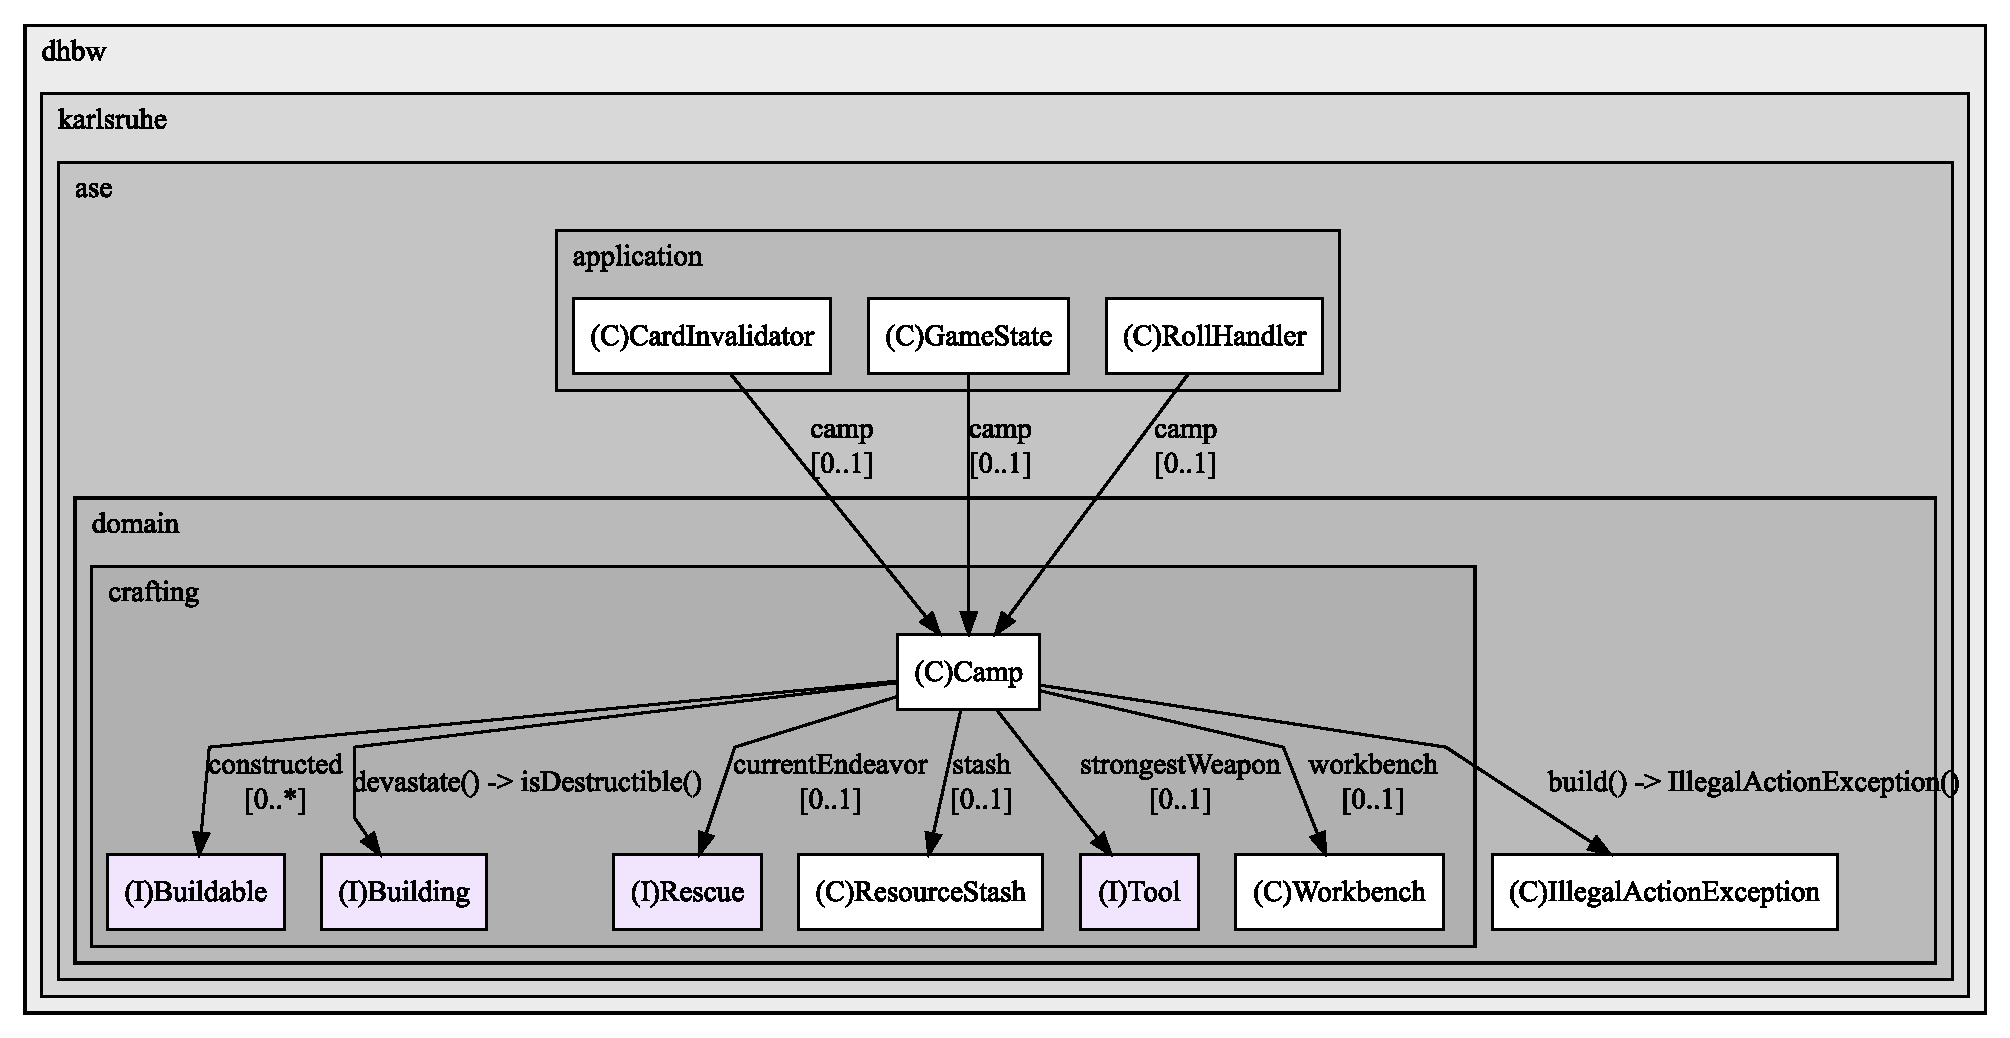
\includegraphics[width=1.\textwidth]{Bilder/Camp_structure.pdf} 
	\caption{UML-Diagramm 1 zum Einhalten der Dependency Rule von \textit{Camp}. }
	\label{fig:dep-camp}
\end{figure} 

\subsubsection{Positiv-Beispiel 2:}

\autoref{fig:dep-game} zeigt ein weiteres positives Beispiel für die Dependency Rule, 
da diese in dieser Softwarearchitektur nicht verletzt wird. Abgebildet ist die Klasse \textit{Game}, 
welche Lediglich von Klassen aus der eigenen Schicht (\textit{application}) und Klassen aus der tieferen 
Schicht \textit{domain} abhängt. Abhänig von Game sind nur Klassen aus der Schicht \textit{plugin},
bzw. dem konkreten \textit{cli}-Plugin. 

\begin{figure}[H]
	\centering
	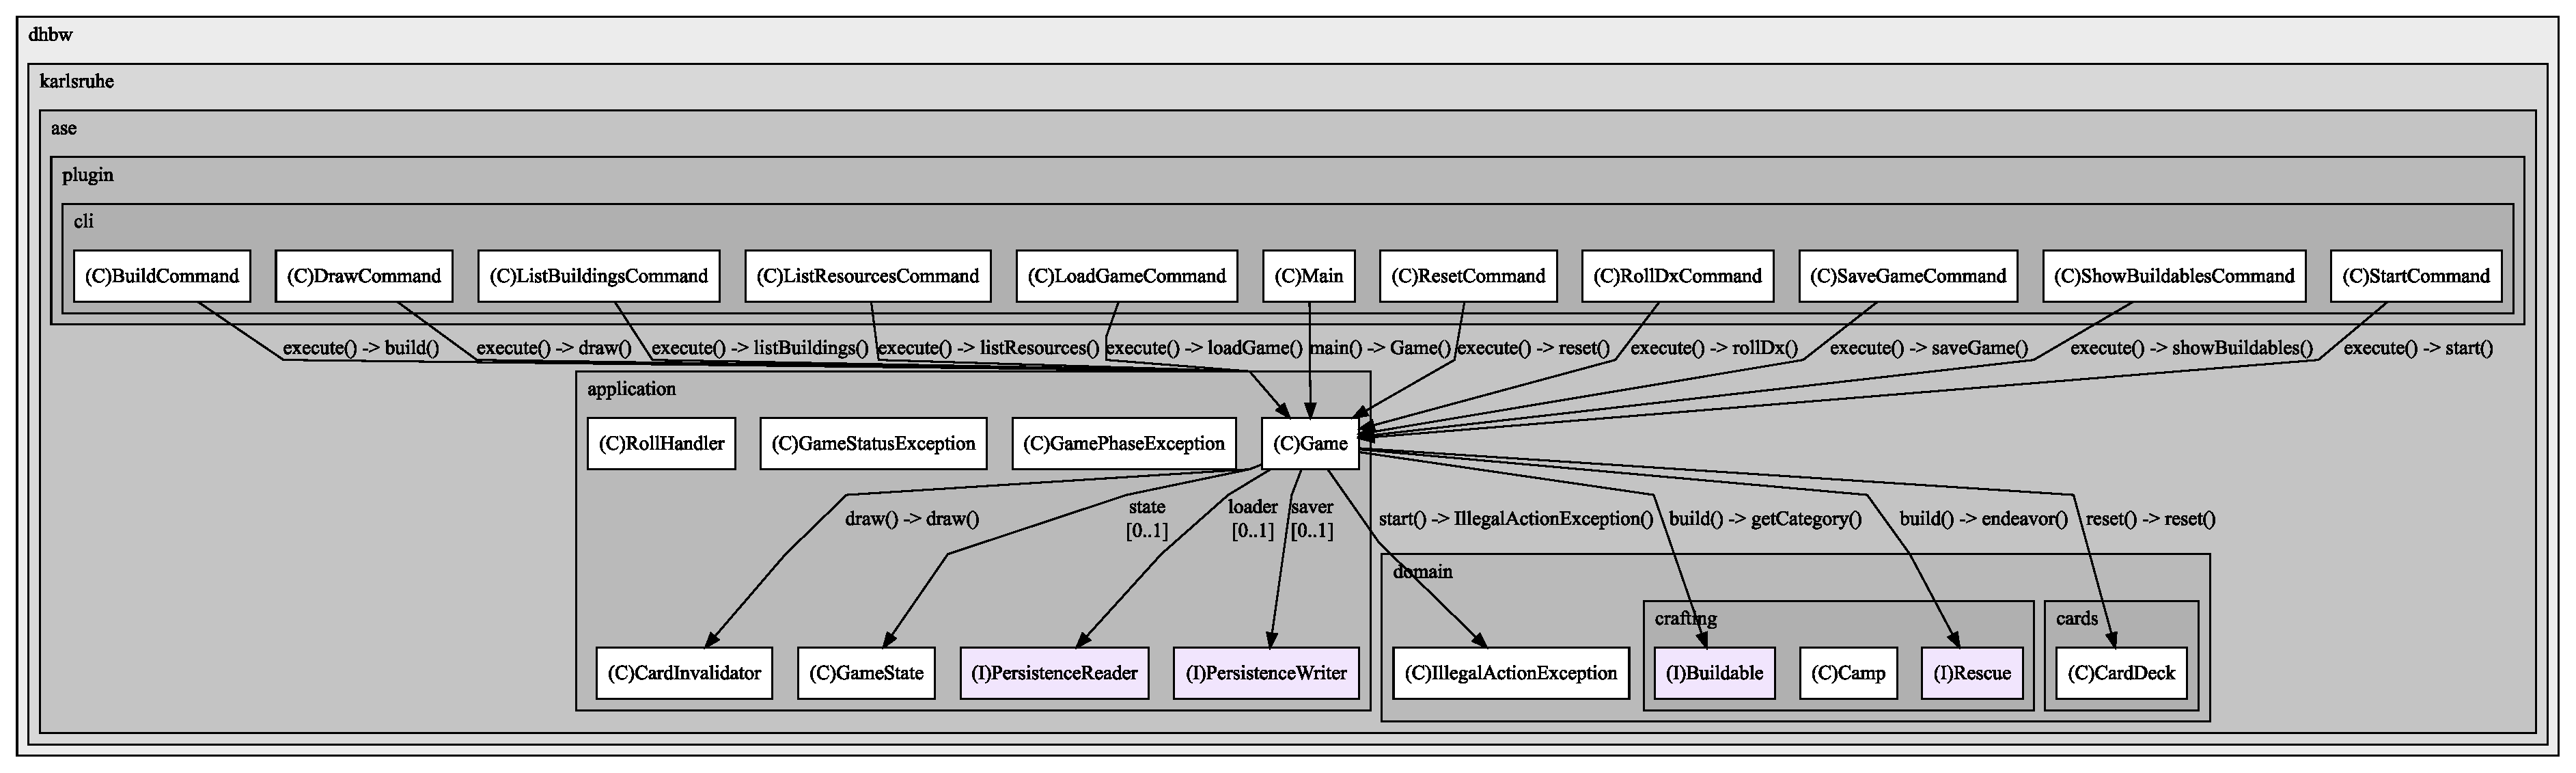
\includegraphics[width=1.05\textwidth]{Bilder/Game_structure.pdf} 
	\caption{UML-Diagramm 2 zum Einhalten der Dependency Rule von \textit{Game}. }
	\label{fig:dep-game}
\end{figure} 


\section{Analyse der Schichten} \label{sec:clean_arch:layers}

In dieser Softwarearchitektur gibt es folgende Schichten aufsteigend sortiert nach Tiefe: 
\texttt{plugin}, \texttt{application}, \texttt{domain} und \texttt{abstraction}.
Hierbei stellt \textit{plugin} die äußerste und \textit{abstraction} die tiefste Schicht dar. 

\subsubsection{Schicht Plugin:}

Bei einem Refactoring der Plugin-Schicht ist aufgefallen, dass viele der (Fehler-)Hinweise, 
die aufgrund von falschem Befehlssyntax oder einem falschen Befehl an den User über das CLI ausgegeben werden, 
keine gemeinsame einheitliche Form aufwiesen, da diese direkt als String ausgegeben wurden. 
Um eine einheitliche Fehlermeldung zu gewährleisten wurde der \textit{ErrorBuilder} eingefügt, 
dessen Aufgabe es ist, die Fehler einheitlich zu formatieren und auszugeben. \autoref{fig:layer-ErrorBuilder} 
zeigt das UML-Klassendiagramm dieser Klasse. Sie wird im gesamten CLI-Plugincode verwendet um (Fehler-)Hinweise 
auszugeben. \\
Über verschiedene Konstruktoren kann ein Grund für den (Fehler-)Hinweis und eine mögliche Abhilfeemfehlung 
eingegeben werden.
Mit der \textit{print}-Methode kann der erzeugte (Fehler-)Hinweis dann formatiert an den User ausgegeben werden. 
Hierzu wird aus Gründen der Testbarkeit an die Funktion \textit{printError} des Proxys \textit{Terminal} delegiert. \\
Diese Klasse befindet sich im Plugin-Layer (insb. im CLI-Plugin), da die konkrete Ausgabe an den User 
in Form von Text von dem CLI abhängt. Die high-level Fehlermeldungen die von den tieferen Schichten über 
Exceptions realisiert sind können von jedem Plugin anders verarbeitet und an den User weitergegeben werden. 
In der CLI funktioniert dies mit dem ErrorBuilder, während es mit einem denkbaren GUI-Plugin über bspw. 
ein Popup funktionieren könnte. Der ErrorBuilder ist lediglich für die Ausgabe an den Nutzer zuständig 
und enhält keine Fehler-Logik und gehört somit in die Plugin-Schicht. 

\begin{figure}[H]
	\centering
	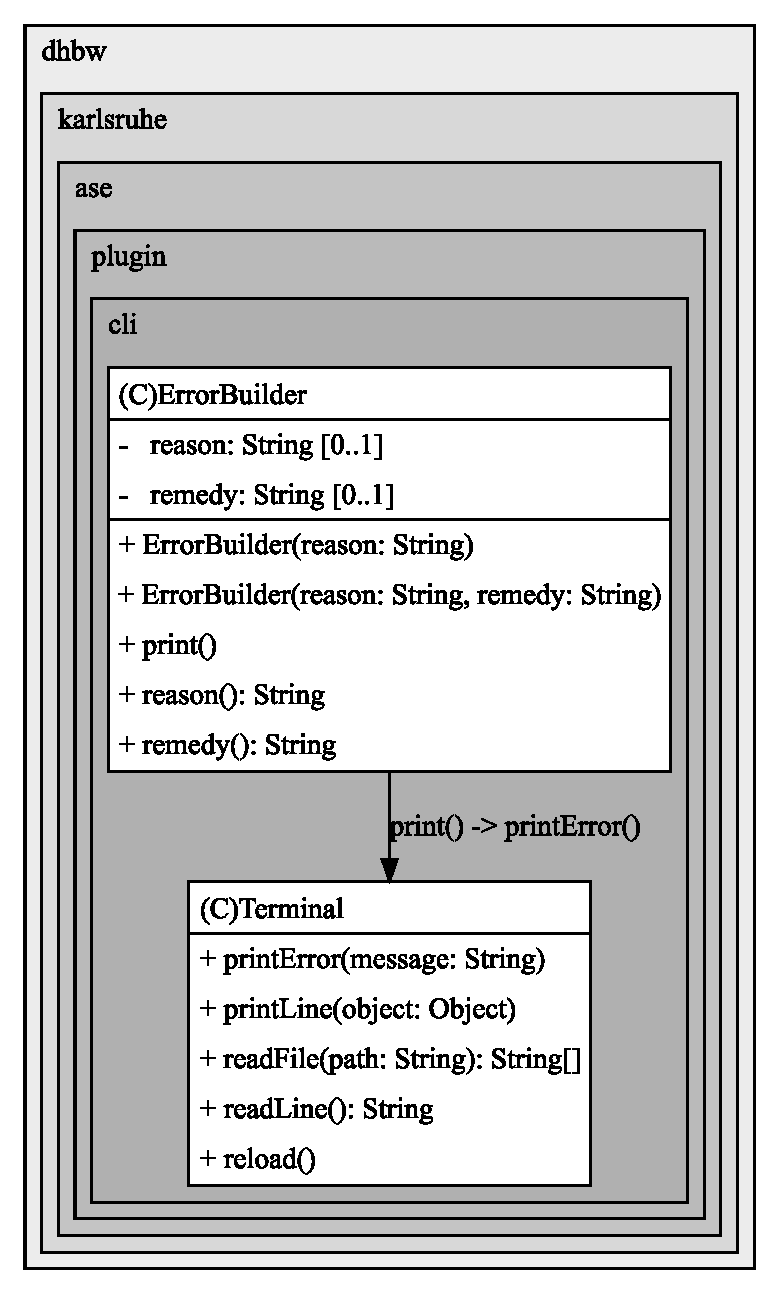
\includegraphics[width=0.5\textwidth]{Bilder/ErrorBuilder_structure.pdf} 
	\caption{Beispielklasse der Plugin-Schicht: ErrorBuilder.}
	\label{fig:layer-ErrorBuilder}
\end{figure} 

\subsubsection{Schicht Domain:}

Der \textit{ResourceStash} ist fester Teil der Domain-Schicht und stellt hier ein Wrapper mit Methodennamen 
in Domänensprache für eine Resource-Deque dar. \autoref{fig:layer-ResourceStash} zeigt das zugehörte UML-Klassendiagramm.
Der ResourceStash beinhaltet und verwaltet alle Ressourcen, die der Spieler im Verlauf des Spiels ansammelt. 
Durch eine Katastrophe oder das Verlieren gegen ein Tier wird der ResourceStash zerstört (\textit{devastate})
und alle ungeschützten Ressourcen gelöscht. Das Erbauen eines \textit{Shack}s\footnote{nicht in der Abb.} 
erlaubt es die obersten $n \in [0;\inf)$ Ressourcen zu schützen (\textit{protectTopMostNResources}), 
sodass diese nach einem \textit{devastate} übrig bleiben. Zusätzlich können Ressourcen hinzugefügt,
konsumiert oder deren Vorhandensein überprüft werden. \textit{Camp} und \textit{Workbench} teilen 
sich eine Referenz auf denselben Stash. \\
Die Klasse ist als Teil des Kartenspiels (der Domäne) im Code natürlich in der Domain-Schicht angesiedelt und 
wird von anderen Domänenklassen genutzt. Es gibt keine Möglichkeit die Klasse in einer der anderen Schichten 
sinnvoll anzusiedeln.

\begin{figure}[H]
	\centering
	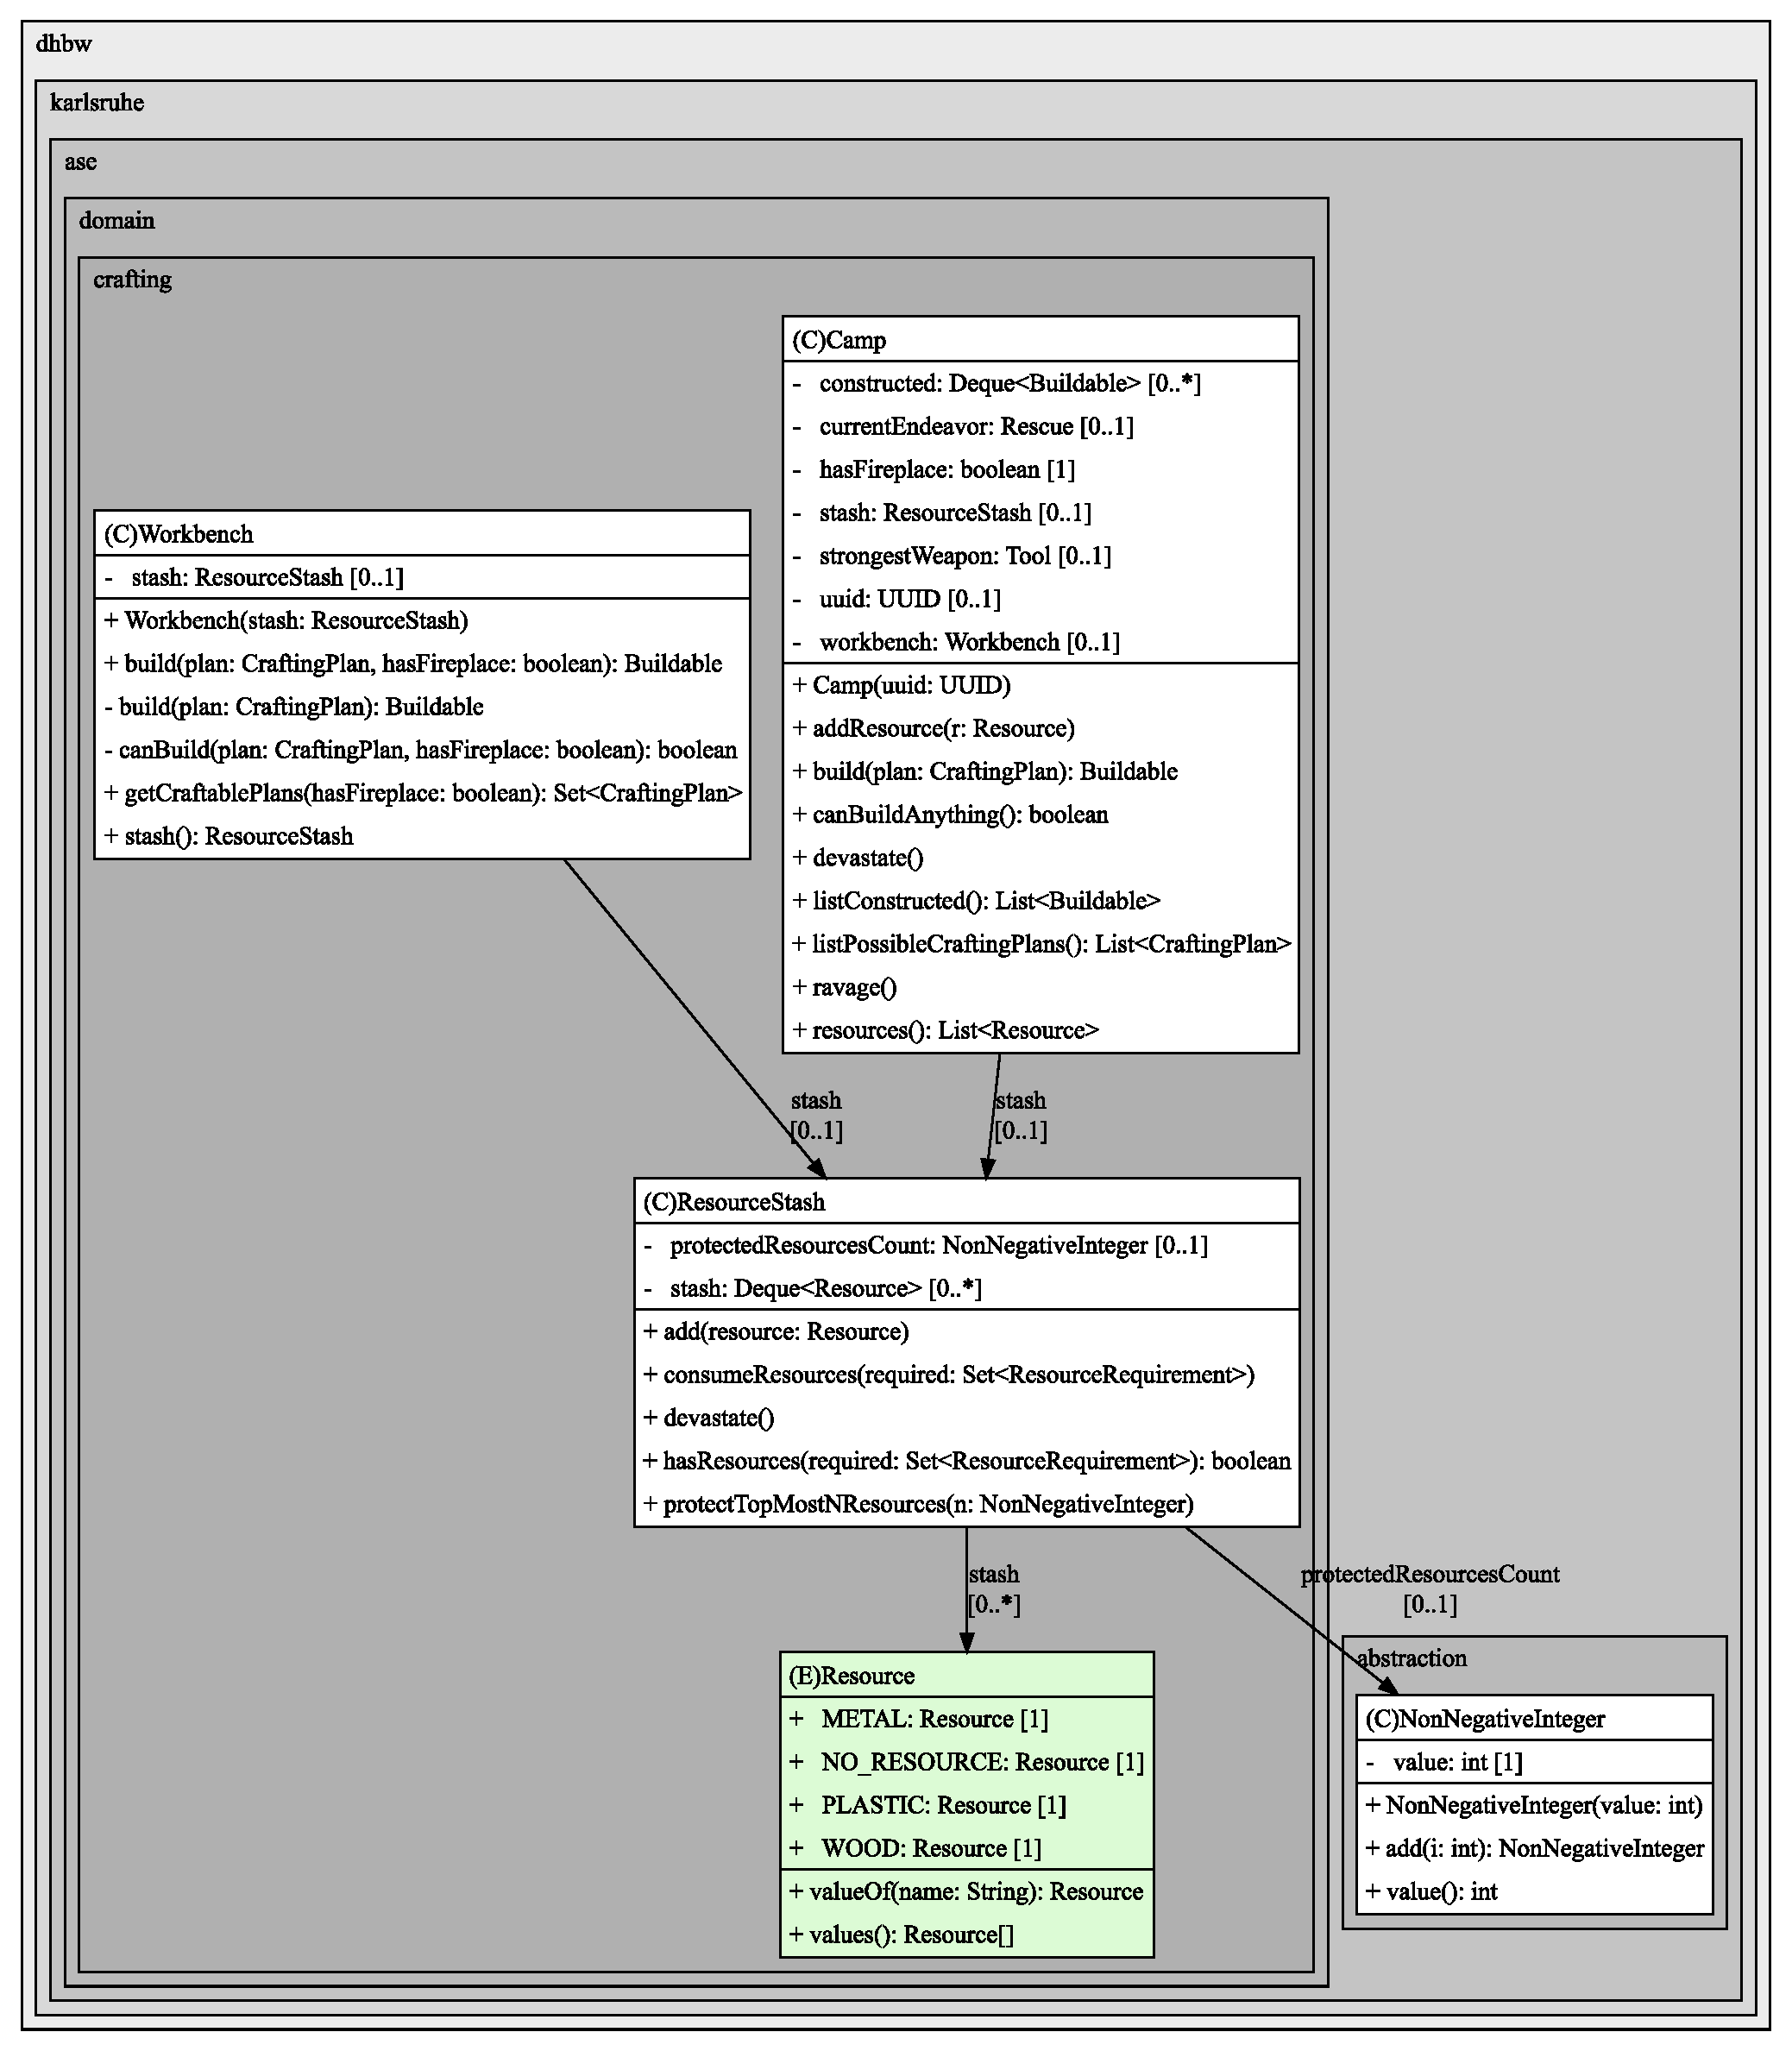
\includegraphics[width=1.05\textwidth]{Bilder/ResourceStash_structure.pdf} 
	\caption{Beispielklasse der Domain-Schicht: ResourceStash.}
	\label{fig:layer-ResourceStash}
\end{figure} 
\chapter{SOLID}

\section{Analyse Single-Responsibility-Principle (SRP)}

\subsubsection{Positiv-Beispiel:}

\begin{wrapfigure}{r}{0.40\textwidth}
	\centering
	\vspace{-30pt} % Manchmal möchte man den oberen Abstand selbst anpassen
	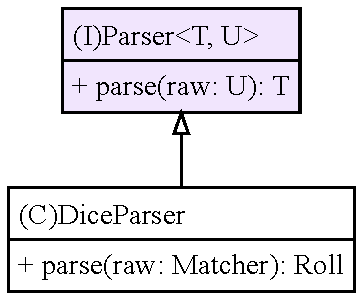
\includegraphics[width=0.30\textwidth]{Bilder/DiceParser_structure.pdf}
	\vspace{-10pt}
	% Das folgende ist ein Trick, um "Abbilgung x.y" in eine
	% eigene Zeile zu packen. Der Text zwischen [ und ] steht
	% im Abbildungsverzeichnis. Der Text darunter wird
	% tatsächlich angezeigt.
	\caption[UML-Diagramm von ase.plugin.cli.parsers.DiceParser.]{\unskip}
	UML-Diagramm von \textit{ase.plugin.cli.parsers.DiceParser}.
	\label{fig:srp-DiceParser}
\end{wrapfigure}

\autoref{fig:srp-DiceParser} zeigt das UML-Klassendiagramm des \textit{DiceParser}, welcher in der Plugin-Schicht
unter \texttt{plugin.cli.parsers} zu finden ist und das Positivbeispiel darstellt. 
Dieser implementiert das \textit{Parser}-Interface aus 
\texttt{plugin.cli}. Die einzige Aufgabe des DiceParsers ist es die Usereingabe zum Erstellen eines Würfelwurfs
aus Text zu parsen und das entsprechende Objekt zu kreieren. Hierzu wird der \textit{Regex}-Matcher, der 
bereits den Syntax überprüft hat an die \textit{parse}-Methode übergeben und daraus die Arugmente extrahiert, 
um den \textit{Roll} zu erstellen.

\subsubsection{Negativ-Beispiel:}

\autoref{fig:srp-RollHandler} zeig das UML-Klassendiagramm des \textit{RollHandler}, welcher in der Applikations-Schicht
die Würfelwürfe für die Rettungen (\textit{Endeavor}) \underline{und} Kämpfe (\textit{Encounter}) bearbeitet. 
Hierbei entscheidet die öffentliche \textit{handle}-Methode, ob es sich um einen Encounter oder ein Endeavor handelt
(dies ist allerdings eigentlich schon bei Aufruf dieser bekannt)
und führt die entsprechende private Methode aus. Die Klasse hat also zwei Aufgaben (Responsibilities). \\
Um dies zu lösen kann einfach die Klasse \textit{RollHandler} in zwei Klassen aufgeteilt werden - 
den \textit{EncounterHandler} und \textit{EndeavorHandler} - die nun jeweils nur noch genau eine Aufgabe haben 
und somit das SRP einhalten, wie \autoref{fig:srp-RollHandler-fixed} zeigt. 

\begin{figure}[H]
	\centering
	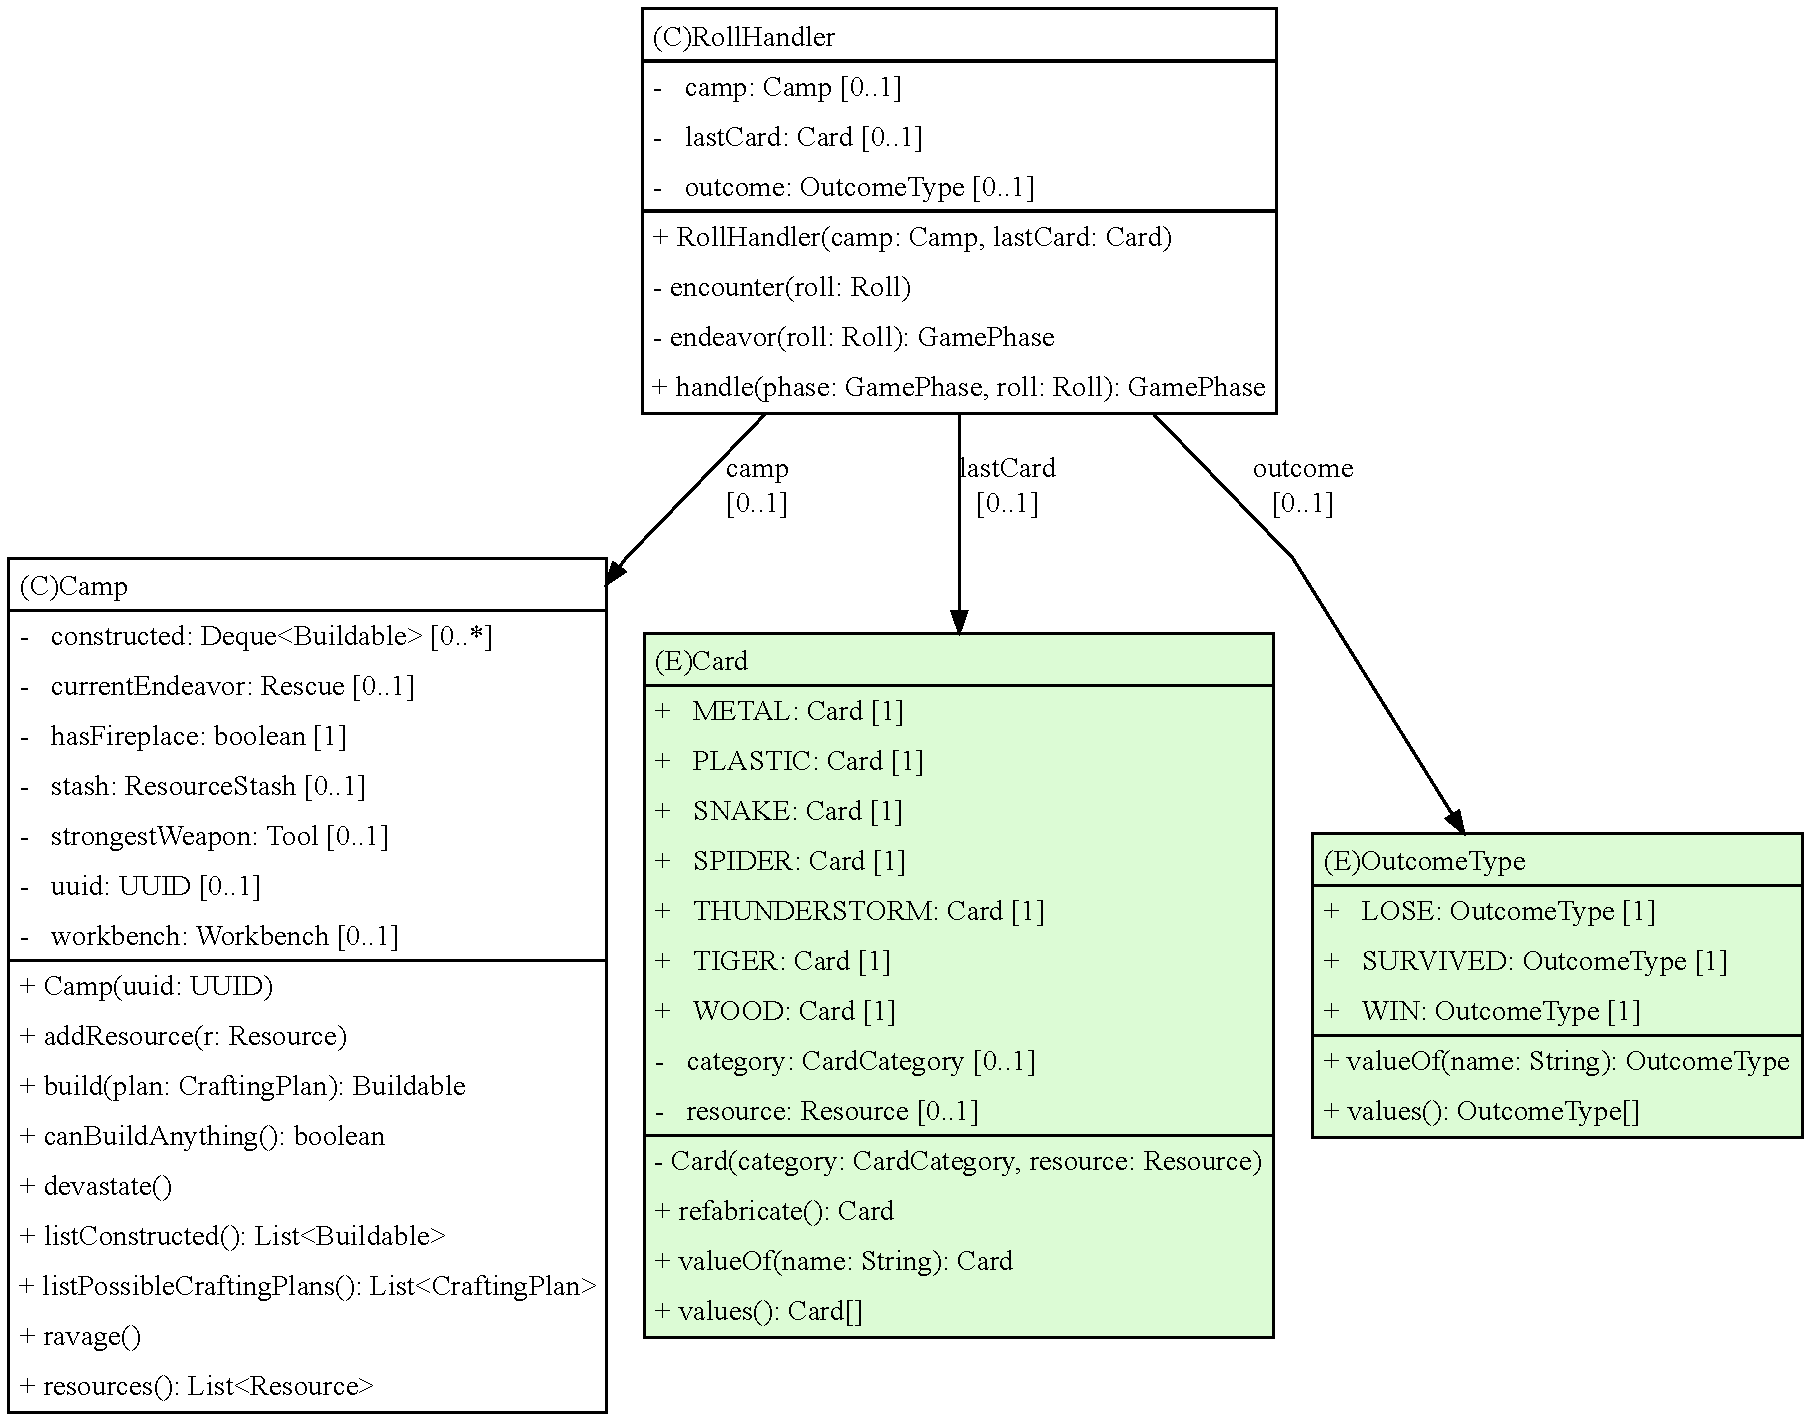
\includegraphics[width=1.\textwidth]{Bilder/RollHandler_structure.pdf} 
	\caption{UML-Diagramm von \textit{application.RollHandler}.}
	\label{fig:srp-RollHandler}
\end{figure} 

\begin{figure}[H]
	\centering
	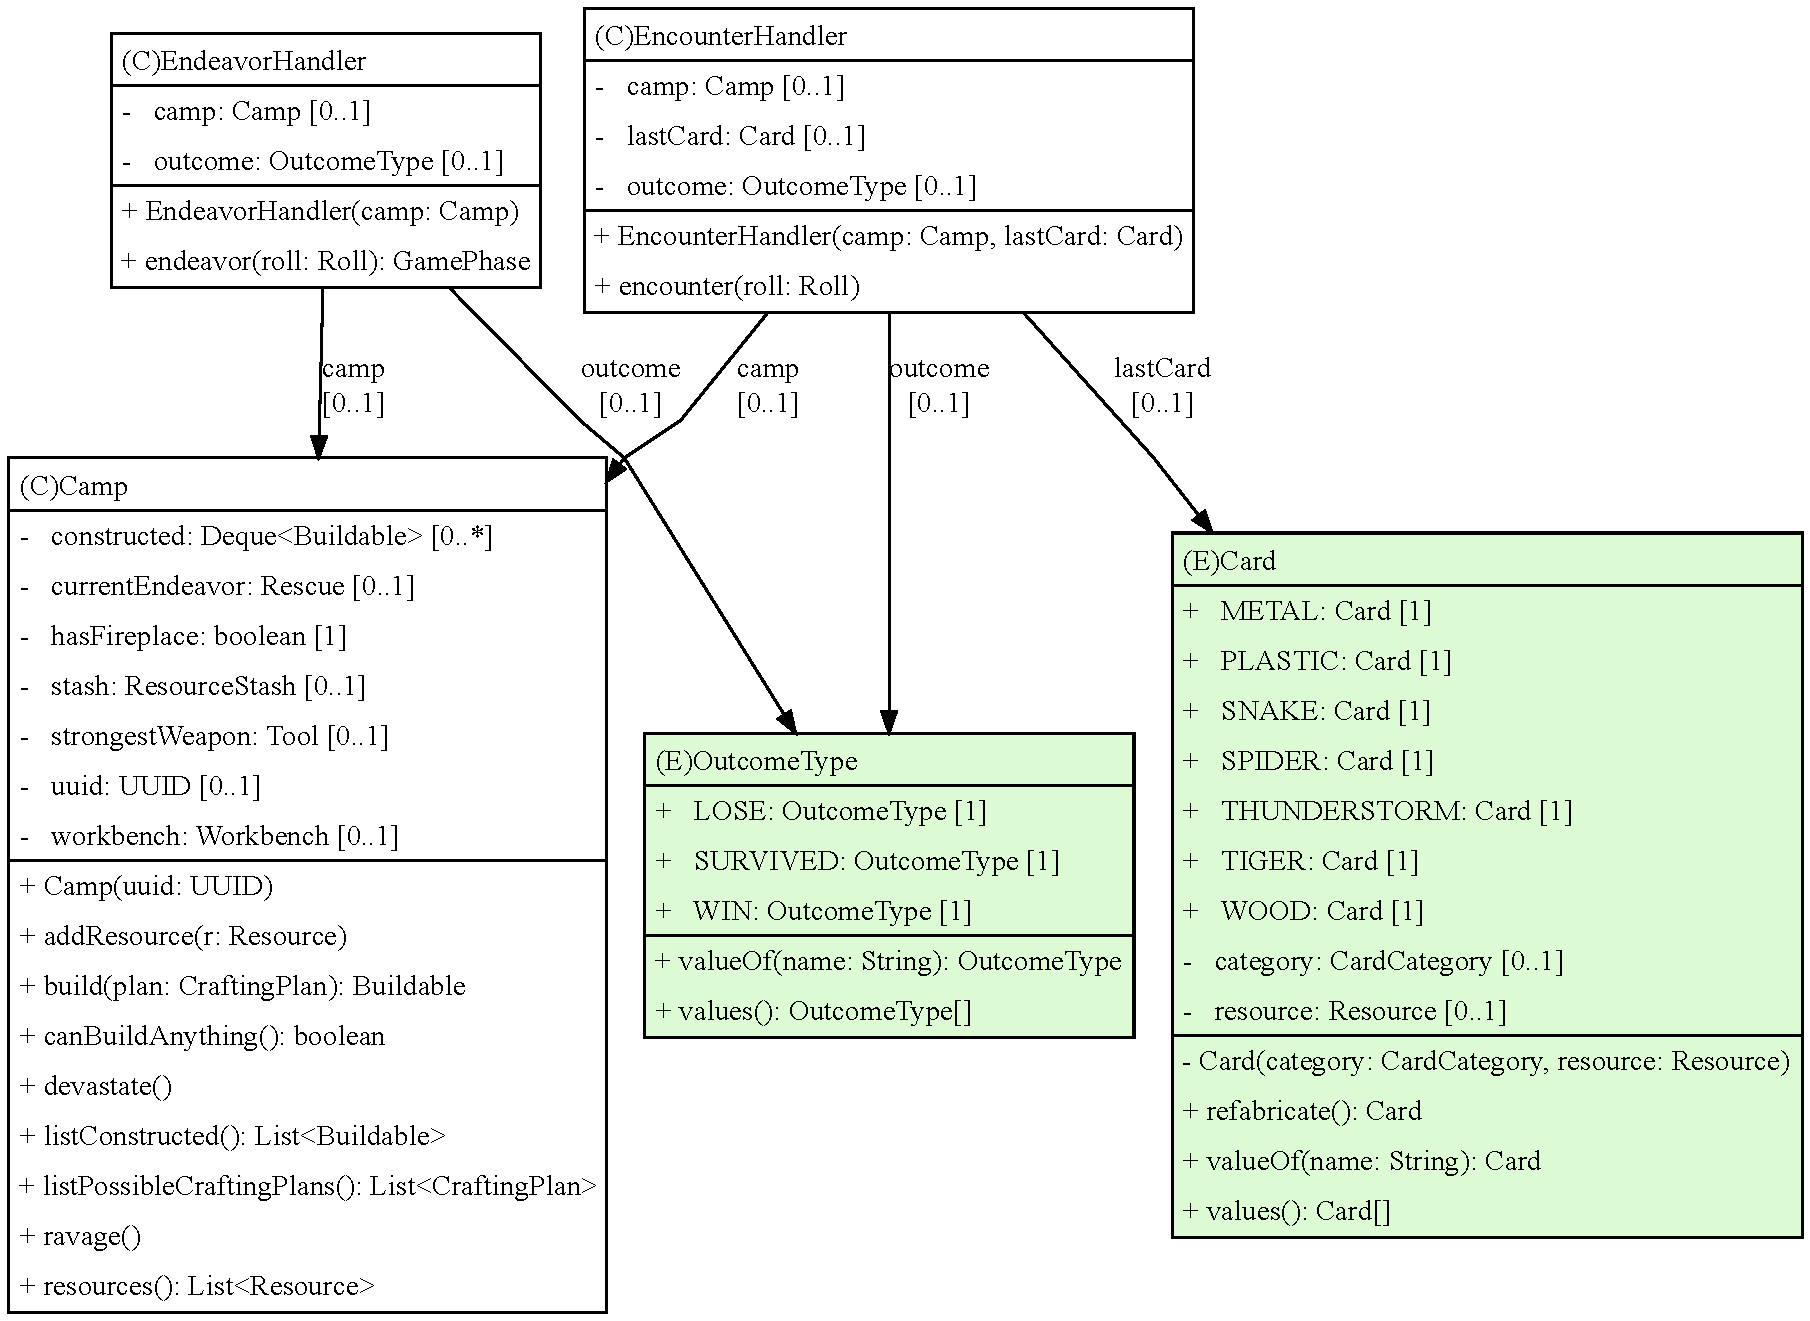
\includegraphics[width=1.\textwidth]{Bilder/RollHandler_fixed_structure.pdf} 
	\caption{\autoref{fig:srp-RollHandler} aufgeteilt in \textit{EndeavorHandler} und \textit{EncounterHandler}.}
	\label{fig:srp-RollHandler-fixed}
\end{figure} 


\section{Analyse Open-Closed-Principle (OCP)}

\subsubsection{Positiv-Beispiel:}

Das Positiv-Beispiel zum OCP wird konstituiert durch das \textit{Command}-Interface aus \texttt{ase.plugin.cli} 
und dessen Implementationen (z.B. \textit{RollDxCommand}) aus \texttt{ase.plugin.cli.commands} wie gezeigt in \autoref{fig:ocp-rolldx}. 
Die Main-Klasse kennt nur das Command-Interface und ruft darauf die \textit{execute}-Methode auf, 
die dann in den unterschiedlichen Command-Implementationen verschiedene Wirkungen auf das übergebene 
\textit{Game} haben. Dies ist auch die Begründung, wieso das OCP hier efüllt wird: Um einen neuen Befehl 
zu implementieren muss lediglich eine weitere Klasse hinzugefügt werden, die das Command-Interface implementiert.
Es muss dazu keine der bestehenden Command-Klassen angepasst oder geändert werden. 

Das OCP ist hier sehr sinnvoll, da für neue Features sehr wahrscheinlich regelmäßig neue Commands hinzugefügt 
werden müssen und dies soll somit möglichst einfach umsetzbar sein und keinen bestehenden Code breaken. 
Zuvor wurden die unterschiedlichen Befehle über zahlreiche \texttt{switch}-Blöcke realisiert 
(siehe z.B. Commit 034a5c28), was Änderungen des Programmcodes an vielen Stellen nötig machte, 
um einen neuen Befehl hinzuzufügen. Außerdem wurden Runtime-Exceptions geworfen, wenn vergessen wurde 
den Code an einer Stelle anzupassen. Durch das neue System müssen \textit{keine} \underline{Änderungen} 
(geschlossen für Änderungen) an vielen Stellen mehr durchgeführt werden, 
sondern nur noch \underline{Additions} durchgeführt werden (offen für Erweiterung).  

\begin{figure}[H]
	\centering
	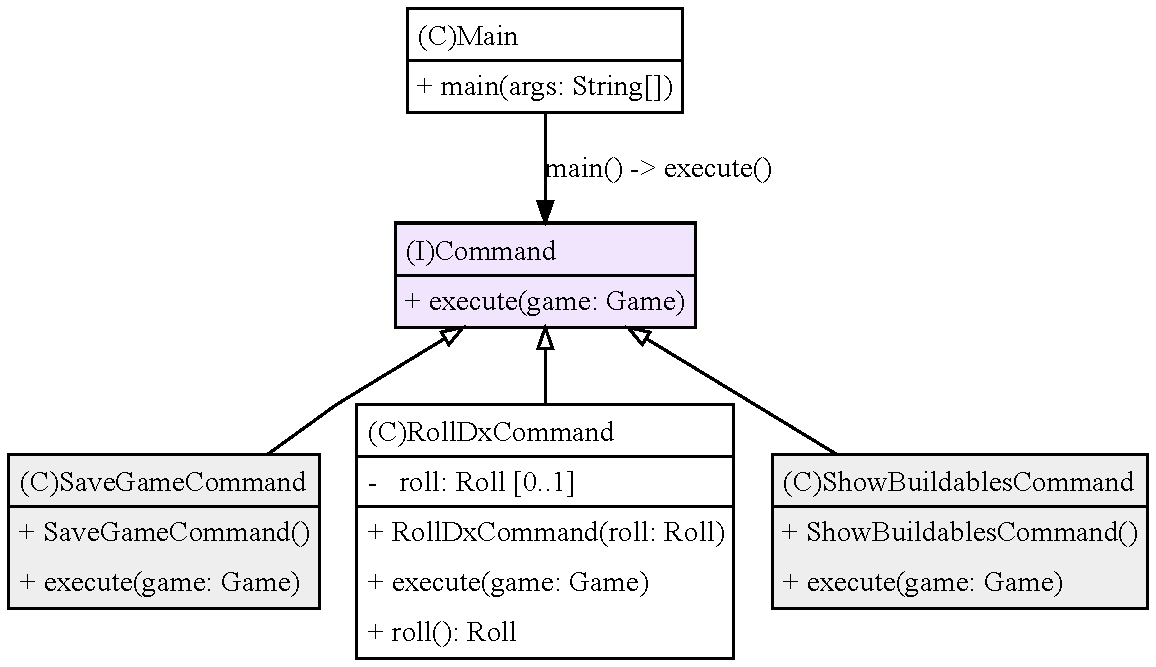
\includegraphics[width=0.7\textwidth]{Bilder/RollDxCommand_structure.pdf} 
	\caption{UML-Klassendiagramm vom \textit{RollDxCommand} und weiteren Commands, 
	wovon die meisten allerdings ausgelassen wurden der Übersichtlichkeit wegen.}
	\label{fig:ocp-rolldx}
\end{figure} 

\subsubsection{Negativ-Beispiel:}


\section{Analyse }


\chapter{Weitere Prinzipien} 

Zunächst wird eine Basisimplementation gegeben, die den Algorithmus zur Subproblemerzeugung und Similarity-Berechnung aus \autoref{sec:alg_comp} umsetzt und diesen dann auf Geschwindigkeit optimiert.

\section{Basisimplementation}

\begin{algorithm}
	\caption{Vereinfachter Algorithmus zum Erstellen der Subprobleme aus den Submodellen}\label{lst:create_sub}
	\begin{algorithmic}[1]
		\Procedure{Create Subproblems}{$F$} 
			\For{$S \in atomicSubmodels$}
				\State $S.graph \gets calculateGraph(S)$
				\State $S.graph \gets reduceGraph(S.graph, F)$
			\EndFor \Comment{$n := |atomicSubmodels|$}
			\While{$|atomicSubmodels| \neq 0$} \Comment{$O(\frac{n(n+1)}{2}) \cdot O(t_{sim}) = O(n^2 \cdot t_{sim})$}
				\State $M \gets selectOne(atomicSubmodels)$
				\State $M.set \gets \emptyset$
				\While{$complexity(M) < minSubproblemComplexity$}
					\State $highestSim \gets -1$					
					\For{$S \in atomicSubmodels$}
						\State $sim \gets computeSim(M, S)$
						\If{$sim > highestSim$}
							\State $mostSimilar \gets S$
							\State $highestSim \gets sim$
						\EndIf
					\EndFor
					\State $M \gets M \cup mostSimilar$
					\State $M.set \gets M.set \cup mostSimilar.set$
					\State $atomicSubmodels \gets atomicSubmodels \setminus mostSimilar$
				\EndWhile
				\State $subproblems \gets subproblems \cup \{M\}$
			\EndWhile		
		\EndProcedure
	\end{algorithmic}
\end{algorithm}


\chapter{Unit Tests} \label{sec:results}


\subsubsection{Mittlere Szenarien}



Die Messungen haben ergeben, dass für alle mittelgroßen Szenarien $s \in S_{Anon_M}$ gilt, dass $t_{sub_{MatFlowG}}(s) < t_{sub_{IdObj}}(s)$. Hierbei haben sich für Identical Objects die Laufzeiten über die 13 Szenarien von $S_{Anon_M}$ zwischen 11s und 1min 39s bewegt, während die Laufzeiten von Material Flow Graph zwischen 1s und 9s lagen. Mit $p=2,744 \cdot 10^{-9}$ ist Material Flow Graph \textit{statistisch signifikant} schneller\footnote{Einseitiger Zwei-Stichproben-t-Test mit unterschiedlicher Varianz; Normalverteilung angenommen; $n=12$; Szenario $z$ mit $t_{sub_{IdObj}}(z) = 1min 39s$ und $t_{sub_{MatFlowG}}(z) = 9s$ als Ausreißer von Test exkludiert.}. 

\begin{table}[ht]
	\centering
	\begin{tabular}{l|l|l|l|l}
		Szenario & $t_{sub_{IdObj}}$ & $t_{sub_{IdMat}}$& $t_{sub_{MatFlowG}}$ & $f_{IdObj \rightarrow MatFlowG}$ \\
		\midrule
		$s_{Krit}$ & 9h 41min 20s & 14min 47s & 3min 31s & $168,15$ \\
		$s_{Ult}$ & 21h & 2h 45min & 15min & $83,\bar{3}$ \\
		
	\end{tabular}
	\caption{Ergebnisse der Laufzeitmessungen von $S_L$ nach verschiedenen Methoden. Außerdem der Beschleunigungsfaktor $f$ von Identical Objects zu Material Flow Graph. Szenario $s_{Ult}$ wurde auf einem Server durchgeführt (Speicherbedarf zu hoch), $s_{Krit}$ auf dem in \autoref{sec:rahmen} beschriebenen Rechner.}
	\label{tab:large_scenarios}
\end{table}

\begin{table}[ht]
	\centering
	\begin{tabular}{l|l|l|l}
		$S_X$ & $\bar{m}_{pre}$ & $\bar{m}_{post}$& $f$ \\
		\midrule
		small & $45,11$ & $5,94$ & $7,6$ \\
		medium & $395,82$ & $120,3$ & $3,29$ \\
		large & $4711,24$ & $50,01$ & $94,19$ \\
	\end{tabular}
	\caption{Durchschnittliche Knotenanzahl vor der Graphenreduktion $\bar{m_{pre}}$, nach der Graphenreduktion $\bar{m_{post}}$ und deren mittlerer Reduktionsfaktor $f$ nach Szenario-Klassen.}
	\label{tab:scenarios_node_nb}
\end{table}
Abschließend zur Untersuchung der praktischen Tests lässt sich also festhalten, dass die erwarteten Ergebnisse erzielt, sowie die theoretischen Überlegungen praktisch bestätigt werden konnten.
\chapter{Domain Driven Design}
\chapter{Refactoring}

\section{Code-Smells} \label{sec:smells}

\subsubsection{Long-Class} 

\autoref{code:long-class-before} und \autoref{code:long-class-after} zeigen den Code eines Long-Class-Code-Smells 
vor (Commit \texttt{174283ab}) und nach (Commit \texttt{b0ce98af}) der Behebung mittels Aufteilen der Klasse 
in drei neue Klassen, die aber jeweils ein gemeinsames Interface (\textit{Parser}) implementieren. \\
Vorher gab es eine \textit{ArgumentParser}-Klasse, die als Methoden-Sammlung für das Parsen von 
\textit{CraftingPlan}s (\textit{parseConstructible}), \textit{Dice} (\textit{parseDice}) 
und \textit{Card}s (\textit{parseCards}) zuständig war. Hierdurch war die Klasse nicht SRP- oder OCP-konform 
und trug den Long-Class-Code-Smell. \\
Dies wurde in \autoref{code:long-class-after} gelöst, 
indem die ArgumentParser-Klasse aufgeteilt wurde in \textit{CardParser}, \textit{CraftingPlanParser} und \textit{DiceParser},
die jeweils das \textit{Parser}-Interface implementieren und somit nur die \textit{parse}-Methode haben. 
(Außerdem wurden die \textit{switch}-Statements gleich mit aufgelöst, aber dieser Code-Smell wird hier nicht betrachtet).
Dadurch wahrt die neue Lösung das SRP und OCP und es ist keine long-class mehr. 

\lstinputlisting[
	label=code:long-class-before,    % Label; genutzt für Referenzen auf dieses Code-Beispiel
	caption=Long-Class-Code-Smell der \textit{ArgumentParser}-Klasse zum Commit \texttt{174283ab}.,
	captionpos=b,               % Position, an der die Caption angezeigt wird t(op) oder b(ottom)
	style=EigenerJavaStyle,   % Eigener Style der vor dem Dokument festgelegt wurde
	firstline=1,                % Zeilennummer im Dokument welche als erste angezeigt wird
	lastline=100                 % Letzte Zeile welche ins LaTeX Dokument übernommen wird
]{Quellcode/long-class-before.java}


\lstinputlisting[
	label=code:long-class-after,    % Label; genutzt für Referenzen auf dieses Code-Beispiel
	caption=Long-Class-Code-Smell behoben durch Aufteilung der Klassen zum Commit \texttt{b0ce98af}.,
	captionpos=b,               % Position, an der die Caption angezeigt wird t(op) oder b(ottom)
	style=EigenerJavaStyle,   % Eigener Style der vor dem Dokument festgelegt wurde
	firstline=1,                % Zeilennummer im Dokument welche als erste angezeigt wird
	lastline=100                 % Letzte Zeile welche ins LaTeX Dokument übernommen wird
]{Quellcode/long-class-after.java}

\subsubsection{Switch-Statement} 

\autoref{code:switch-before} und \autoref{code:switch-after} zeigen den Code eines Switch-Statement-Code-Smells 
vor (Commit \texttt{dd2a39d2}) und nach (Commit \texttt{a0e99692}) der Behebung mittels Einführung einer 
Map, die das Zählen dynamisch übernimmt. \\ 
Vorher gab es nur die \textit{CardDeck}-Klasse, die mit der \textit{isValid}-Methode überprüft, 
ob die Karten-Konfiguration (also die Anzahl der verschiedenen Karten im Deck) zulässig ist. 
Das Zählen der Karten funktionierte über ein Switch-Statement, welches einen explizit für diesen 
Kartentyp vorgesehenen Zähler inkrementierte, wenn die Karte bei Iteration über die Sammlung von eben diesem Typ war.
Der Vergleich auf Validität erfolgte über eine Kaskade von verundeten Gleichheitstests mit den erwünschten Werten. 
Diese Methode war furchtbar unerweiterbar. \\
Die Lösung in \autoref{code:switch-after} funktioniert so: Es wurde das neue VO \textit{CardDeckConfiguration} 
eingeführt, welches eine immutable Map von Card -> Integer mappt und ermöglicht zu überprüfen, ob zwei 
CardDeckConfigurations wertetechnisch gleich sind (\textit{record}'s implizites \textit{equals}). Zur 
besseren Vergleichbarkeit hat CardDeckConfiguration die \textit{withoutZeroOccurrences}-Methode, um Karten, 
die null Mal vorkommen, zu entfernen. CardDeck hat nun das Attribut \textit{config}, welches die erwünschte 
CardDeckConfiguration beinhaltet. Der Switch in \textit{isValid} wurde nun ersetzt, indem durch einen 
Loop über das CardDeck die Anzahl an Karten eines Typs dynamisch über eine Map-Struktur gezählt werden (Kartentyp 
ist der Schlüssel) und dann schließlich die Ist- und Soll-Konfiguration über ein \textit{equals}-Aufruf verglichen 
werden. Hierdurch wurde der Switch-Code-Smell entfernt und CardDeck ist nun OCP-konform, da nichts an der Klasse 
(also der frühere Switch und die Zähler pro Kartentyp und deren Vergleich) geändert werden muss, wenn ein neuer 
Kartentyp hinzugefügt wird.   

\lstinputlisting[
	label=code:switch-before,    % Label; genutzt für Referenzen auf dieses Code-Beispiel
	caption=Switch-Statement-Code-Smell der \textit{CardDeck}-Klasse zum Commit \texttt{dd2a39d2}.,
	captionpos=b,               % Position, an der die Caption angezeigt wird t(op) oder b(ottom)
	style=EigenerJavaStyle,   % Eigener Style der vor dem Dokument festgelegt wurde
	firstline=1,                % Zeilennummer im Dokument welche als erste angezeigt wird
	lastline=100                 % Letzte Zeile welche ins LaTeX Dokument übernommen wird
]{Quellcode/switch-before.java}


\lstinputlisting[
	label=code:switch-after,    % Label; genutzt für Referenzen auf dieses Code-Beispiel
	caption=Switch-Statement-Code-Smell behoben durch neue \textit{DeckConfiguration}-Klasse und Map zum Zeitpunkt des Commit \texttt{a0e99692}.,
	captionpos=b,               % Position, an der die Caption angezeigt wird t(op) oder b(ottom)
	style=EigenerJavaStyle,   % Eigener Style der vor dem Dokument festgelegt wurde
	firstline=1,                % Zeilennummer im Dokument welche als erste angezeigt wird
	lastline=100                 % Letzte Zeile welche ins LaTeX Dokument übernommen wird
]{Quellcode/switch-after.java}

\section{2 Refactorings}

\subsubsection{Extract-Method}

\autoref{fig:extract-before} und \autoref{code:extract-method-before} zeigen die \textit{isValid}-Methode 
der \textit{CardDeck}-Klasse\footnote{Wie in \autoref{sec:smells}.}
\underline{vor} dem \textit{Extract-Method}-Refactoring und \autoref{fig:extract-after} und \autoref{code:extract-method-after} \underline{nach}
dem Refactoring durch \underline{Commit \texttt{cb55ad97}}. \\
Extract-Method wurde hier angewandt, um die Lesbarkeit der \textit{isValid}-Methode deutlich zu erhöhen, da für den 
ersten Teil nicht direkt klar war, was passiert, wodurch fast ein Code-Comment-Smell benötigt worden wäre, ohne Method-Extraction. 
Nun ist in der isValid-Methode klar, was im ersten Zeil (zählen der eigenen Karten) und im zweiten Teil (Vergleich mit der Soll-Konfiguration) 
passiert. Außerdem ist die neue extrahierte Methode \textit{countCardOccurrences} eine recht allgemeine Methode, die ggf. in Zukunft 
noch an anderer Stelle verwendet werden kann, um Code-Duplication zu verhindern. 

\lstinputlisting[
	label=code:extract-method-before,    % Label; genutzt für Referenzen auf dieses Code-Beispiel
	caption=\textit{isValid}-Methode \underline{vor} Method-Extraction (aus u.a. Commit \texttt{a0e99692}). Vgl. \autoref{code:switch-after}.,
	captionpos=b,               % Position, an der die Caption angezeigt wird t(op) oder b(ottom)
	style=EigenerJavaStyle,   % Eigener Style der vor dem Dokument festgelegt wurde
	firstline=35,                % Zeilennummer im Dokument welche als erste angezeigt wird
	lastline=50                 % Letzte Zeile welche ins LaTeX Dokument übernommen wird
]{Quellcode/switch-after.java}

\begin{figure}[H]
	\centering
	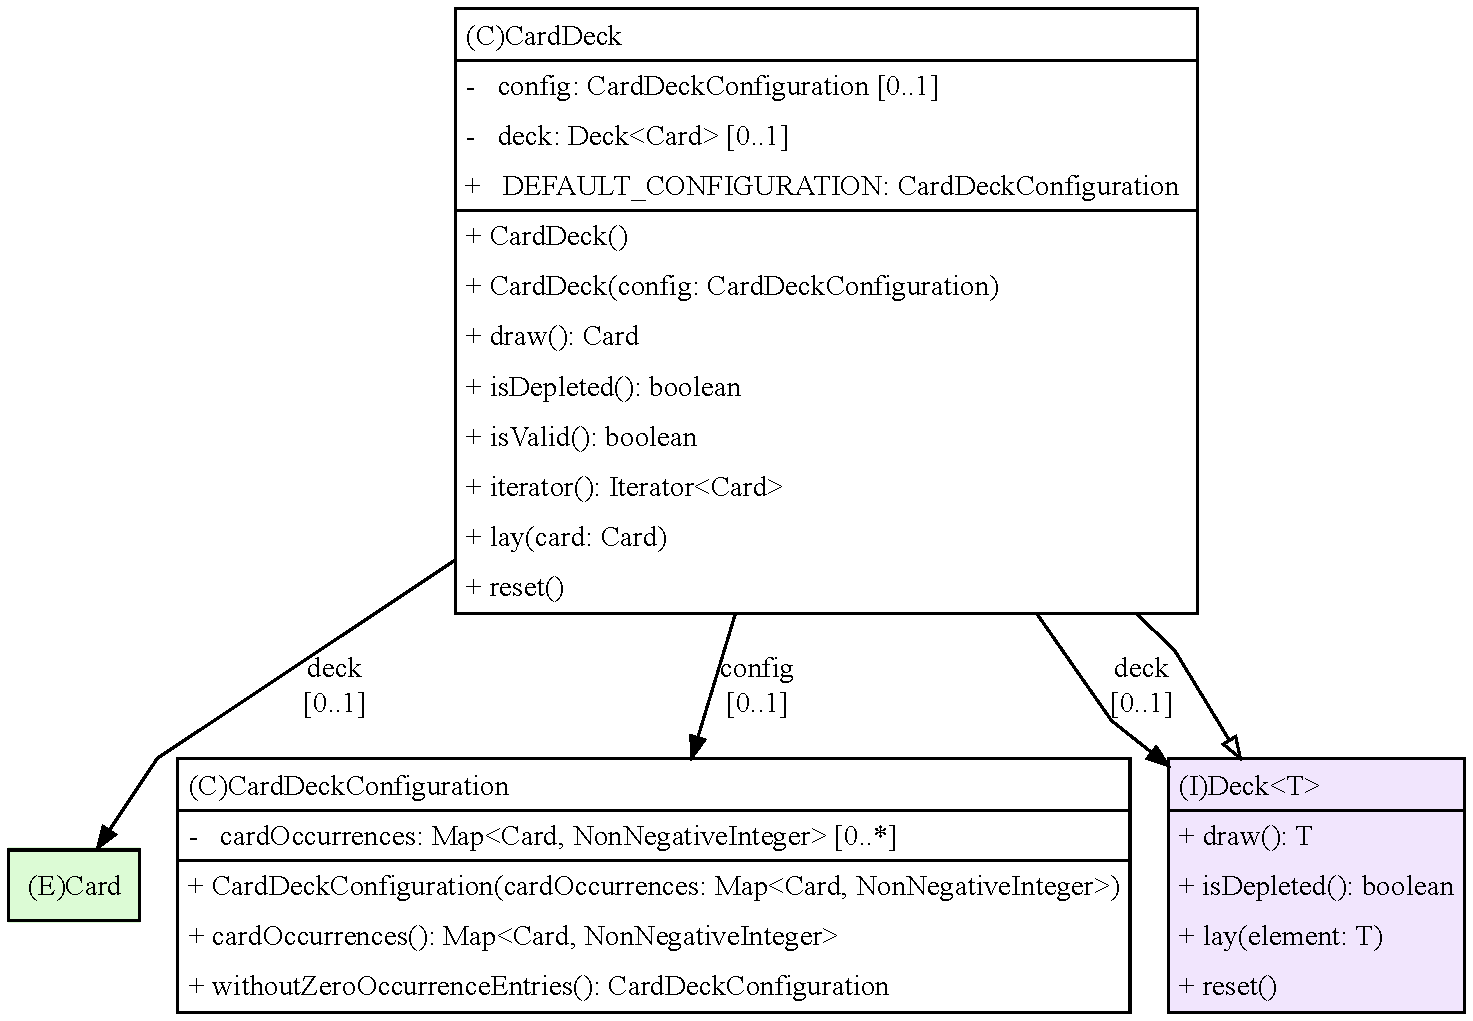
\includegraphics[width=0.85\textwidth]{Bilder/CardDeck_extract-before_structure.pdf} 
	\caption{UML-Diagramm von \textit{CardDeck} \underline{vor} der Method-Extraction.}
	\label{fig:extract-before}
\end{figure} 

\lstinputlisting[
	label=code:extract-method-after,    % Label; genutzt für Referenzen auf dieses Code-Beispiel
	caption=\underline{Nach} Method-Extraction der Methode \textit{countCardOccurrences} aus der \textit{isValid}-Methode in Commit \texttt{cb55ad97}.,
	captionpos=b,               % Position, an der die Caption angezeigt wird t(op) oder b(ottom)
	style=EigenerJavaStyle,   % Eigener Style der vor dem Dokument festgelegt wurde
	firstline=1,                % Zeilennummer im Dokument welche als erste angezeigt wird
	lastline=100                 % Letzte Zeile welche ins LaTeX Dokument übernommen wird
]{Quellcode/extract-method-after.java}

\begin{figure}[H]
	\centering
	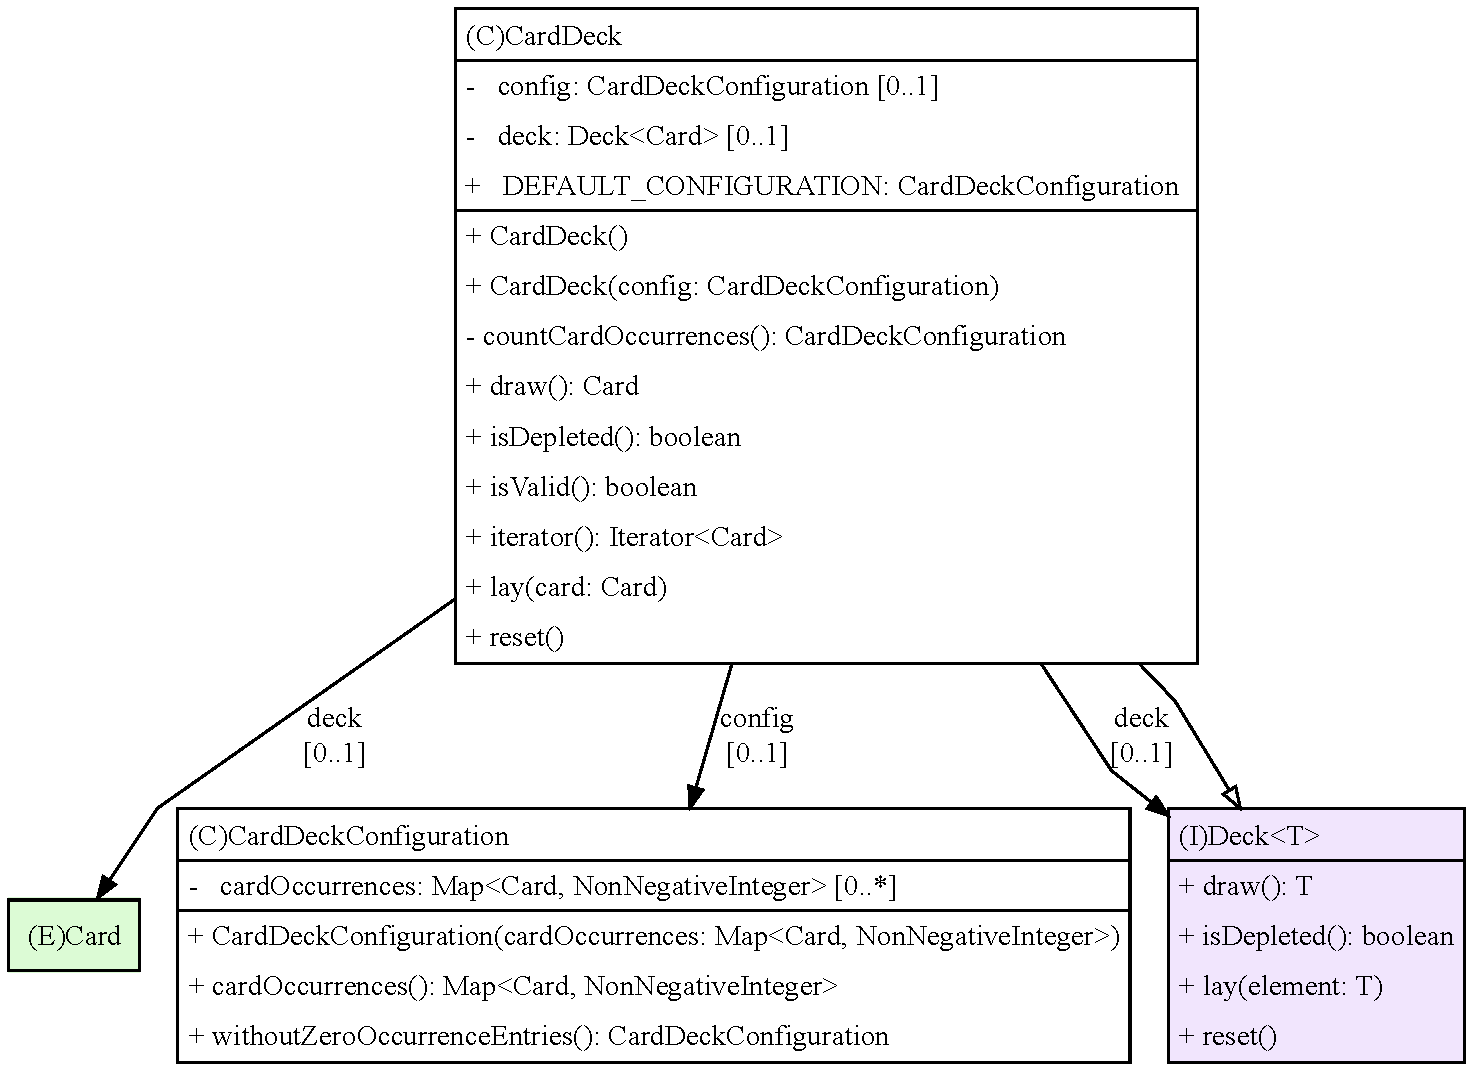
\includegraphics[width=0.85\textwidth]{Bilder/CardDeck_extract-after_structure.pdf} 
	\caption{UML-Diagramm von \textit{CardDeck} \underline{nach} der Method-Extraction durch Commit \texttt{cb55ad97}. 
	Beachte die neue private Methode \textit{countCardOccurrences} in \textit{CardDeck}.}
	\label{fig:extract-after}
\end{figure} 



\subsubsection{Replace-Temp-with-Query (RTQ)}

\autoref{fig:rtq-before} und \autoref{code:rtq-before} zeigen die \textit{execute}-Methode 
der \textit{StartCommand}-Klasse
\underline{vor} dem \textit{Replace-Temp-with-Query-(RTQ)}-Refactoring und \autoref{fig:rtq-after} und \autoref{code:rtq-after} \underline{nach}
dem Refactoring durch \underline{Commit \texttt{827cd843}}. \\
Das Extrahieren der Berechnung des \textit{CardDeck} von der \textit{execute}-Methode in die \textit{deckFrom}-Methode 
hilft dabei, dass die execute-Methode das SRP einhält und nur noch zuständig ist, den Output der \textit{start}-Methode 
der \textit{Game}-Klasse an den User auszugeben. Außerdem wird dadurch der \textit{Long-Method}-Code-Smell der 
\textit{execute}-Methode beseitigt.

\lstinputlisting[
	label=code:rtq-before,    % Label; genutzt für Referenzen auf dieses Code-Beispiel
	caption=\textit{execute}-Methode \underline{vor} RTQ-Refactoring.,
	captionpos=b,               % Position, an der die Caption angezeigt wird t(op) oder b(ottom)
	style=EigenerJavaStyle,   % Eigener Style der vor dem Dokument festgelegt wurde
	firstline=1,                % Zeilennummer im Dokument welche als erste angezeigt wird
	lastline=100                 % Letzte Zeile welche ins LaTeX Dokument übernommen wird
]{Quellcode/query-before.java}

\begin{figure}[H]
	\centering
	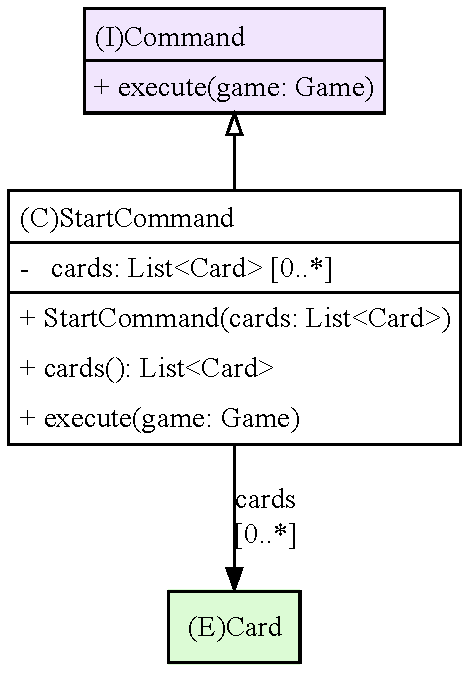
\includegraphics[width=0.4\textwidth]{Bilder/StartCommand_before_structure.pdf} 
	\caption{UML-Diagramm von \textit{StartCommand} \underline{vor} dem RTQ-Refactoring.}
	\label{fig:rtq-before}
\end{figure} 

\lstinputlisting[
	label=code:rtq-after,    % Label; genutzt für Referenzen auf dieses Code-Beispiel
	caption=\textit{execute}-Methode und \textit{deckFrom}-Methode \underline{nach} RTQ-Refactoring in Commit \texttt{827cd843}.,
	captionpos=b,               % Position, an der die Caption angezeigt wird t(op) oder b(ottom)
	style=EigenerJavaStyle,   % Eigener Style der vor dem Dokument festgelegt wurde
	firstline=1,                % Zeilennummer im Dokument welche als erste angezeigt wird
	lastline=100                 % Letzte Zeile welche ins LaTeX Dokument übernommen wird
]{Quellcode/query-after.java}

\begin{figure}[H]
	\centering
	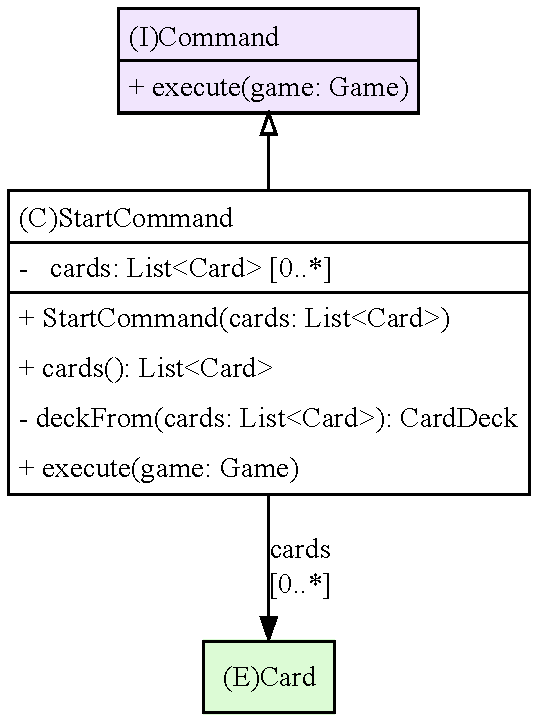
\includegraphics[width=0.4\textwidth]{Bilder/StartCommand_after_structure.pdf} 
	\caption{UML-Diagramm von \textit{StartCommand} \underline{nach} dem RTQ-Refactoring 
	durch Extraktion des Erstellens eines neuen Decks in Commit \texttt{827cd843}. 
	Beachte die neue private Methode \textit{countCardOccurrences} in \textit{CardDeck}.}
	\label{fig:rtq-after}
\end{figure} 
\chapter{Entwurfsmuster}

\section{Entwurfsmuster: Observer-Pattern}

\autoref{fig:observer} zeigt das Observer-Pattern, wobei ein \textit{GameEndObserver} von einem \textit{GameEndObservable} benachrichtigt 
wird, wenn das Spielende erreicht ist und mit einem \textit{GameResult} abgeschlossen wird. Das UML zeigt das 
konkrete GameEndObservable \textit{GameState}, welches seine GameEndObservers updated, wenn das GameResult über einen 
Setter geändert wird. Der konkrete GameEndObserver \textit{GameEndReporter} aus der Plugin-Schicht gibt dann 
das Spielergebnis an den User aus. Hierfür wird der GameEndReporter in der \textit{main}-Methode erzeugt und über 
DI an die höhere Schicht weitergegeben. \\ 
Das Observer-Pattern ist hier sehr sinnvoll, da das Spielende ein Zustand ist, 
der über viele verschiedene Wege und User-Befehle erreicht werden kann, wie zum Beispiel das Ziehen der letzten 
Karte, ohne dass noch eine Aktion möglich ist, oder der Spieler mit dem letzten möglichen Endeavor nicht erfolgreich ist usw. 
Daher ist es sinnvoll dies über ein Event abzuwickeln, damit nicht viele verschiedene Commands separat auf Spielende checken müssen, 
was auch gegen das SRP gehen würde. Außerdem erlaubt es eine sehr flexible Erweiterbarkeit, wenn zum Beispiel ein 
Highscore-Mechanismus eingebaut werden soll, der am Spielende die benötigten Züge abspeichert.      

\begin{figure}[H]
	\centering
	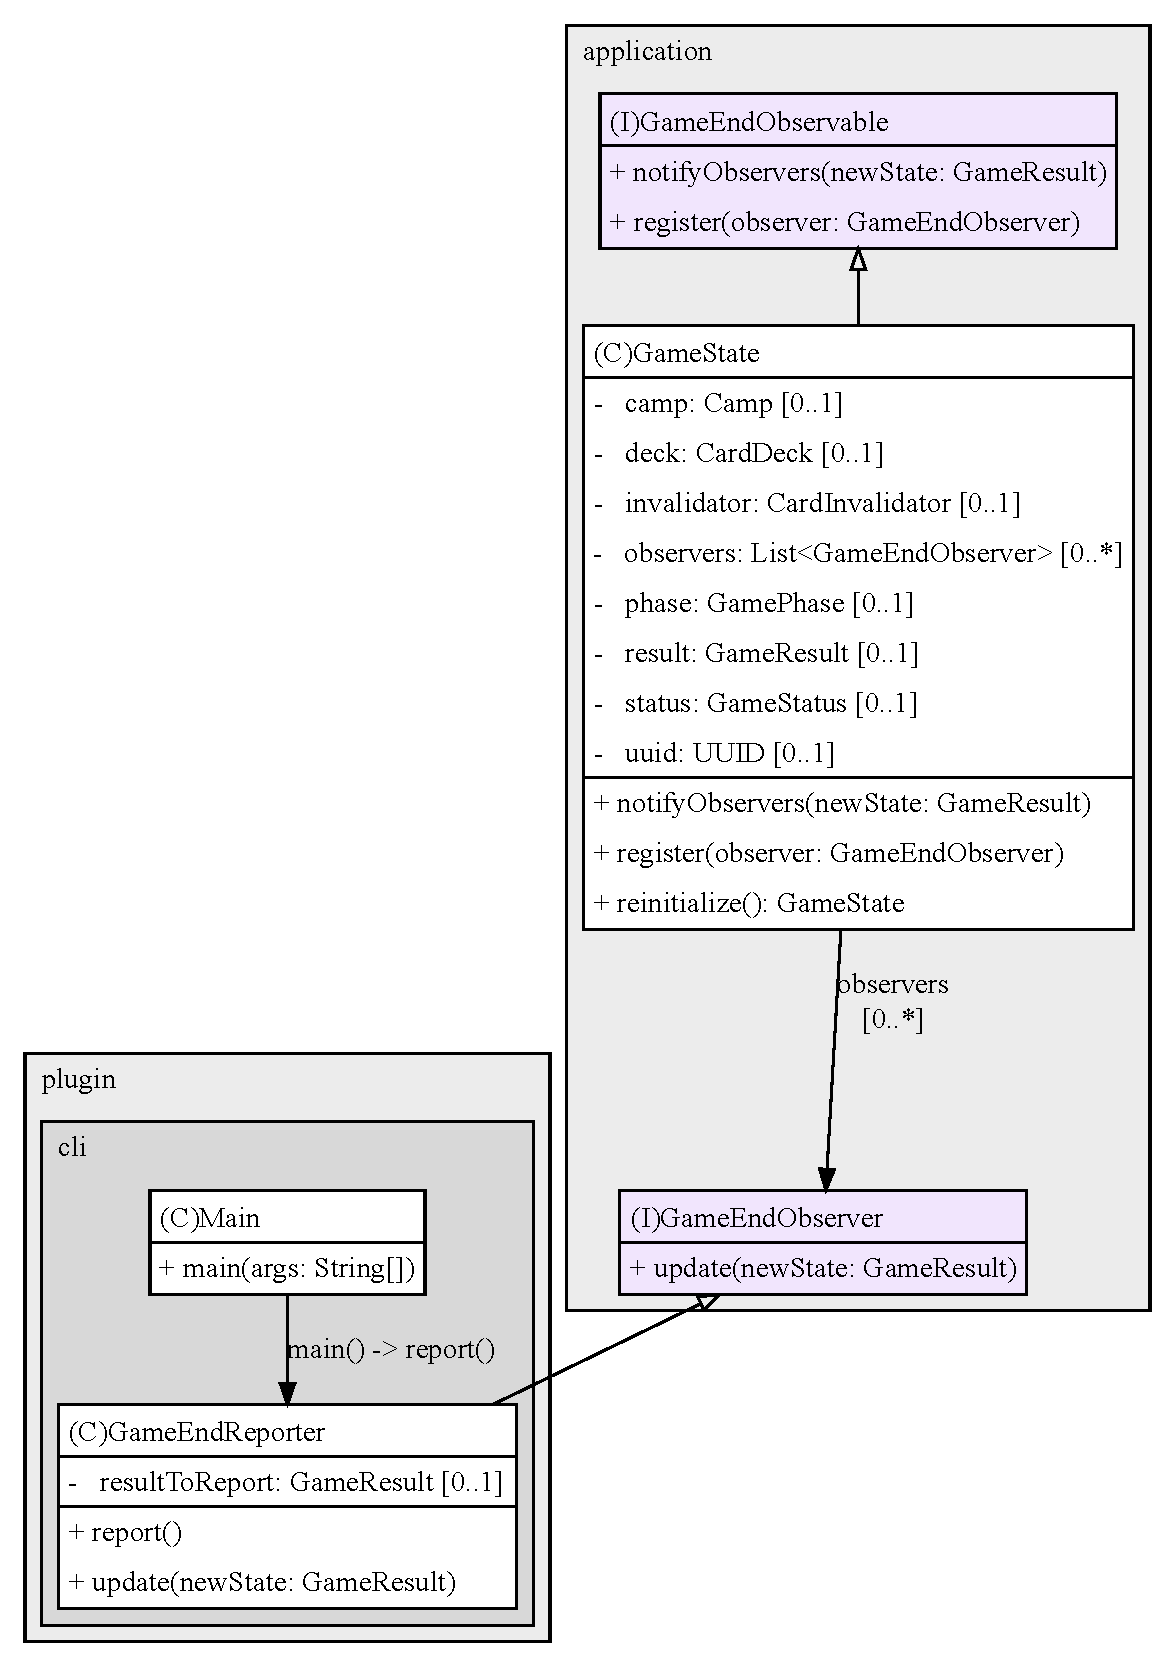
\includegraphics[width=0.6\textwidth]{Bilder/GameEndObserver_structure.pdf} 
	\caption{UML-Diagramm des Observer-Patterns zwischen \textit{GameState} und \textit{GameEndReporter}.}
	\label{fig:observer}
\end{figure} 

\section{Entwurfsmuster: Strategie}

\autoref{fig:strategy} zeigt das Stragie-Entwurfsmuster für die Logik der unterschiedlichen Endeavor-Möglichkeiten. 
Hierzu hält der Anwender \textit{RollHandler} eine Referenz auf die Strategie \textit{Rescue}, für die die 
Methode \textit{endeavor} implementiert werden muss. Die konkreten Strategien \textit{GuaranteedRescue} und \textit{PossibleRescue}
implementieren das Interface und können so flexibel von dem Anwender RollHandler verwendet werden. \\ 
Das Pattern ergibt hier sehr viel Sinn, da der RollHandler die konkrete Berechnung, ob das Endeavor geglückt ist oder nicht, 
nicht selbst durchführen muss, bzw. davon nichts wissen muss. Das unterstützt sehr stark das OCP, SRP und geringe Kopplung. 
Sollte eine weitere Form der Rescue eingeführt werden und möglich werden, ist das Programm so sehr flexibel und einfach 
erweiterbar.  

\begin{figure}[H]
	\centering
	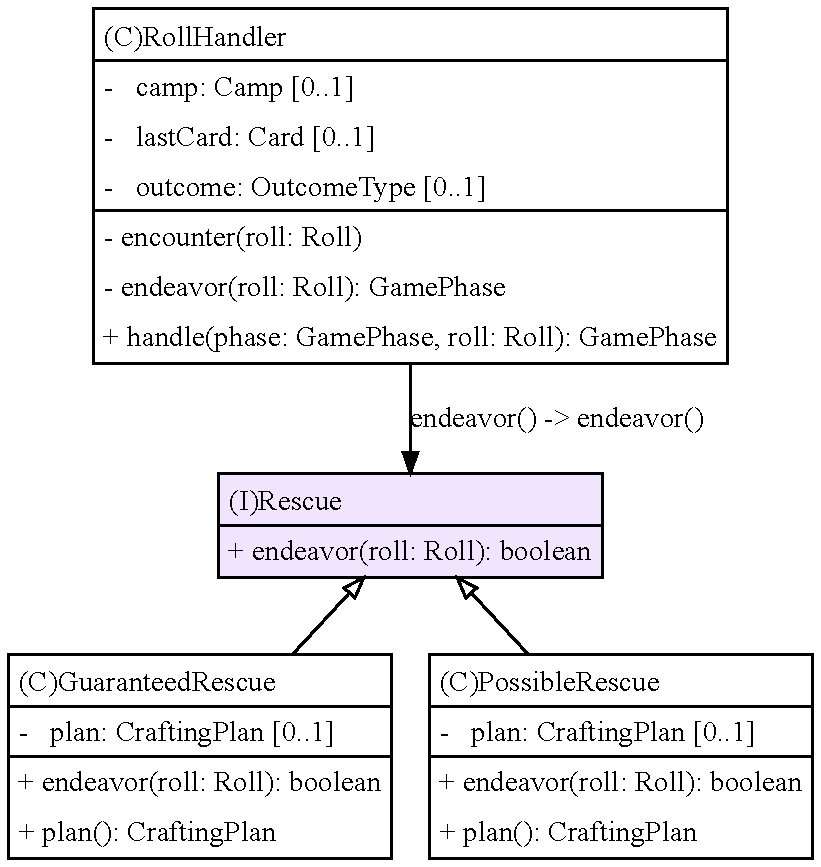
\includegraphics[width=0.5\textwidth]{Bilder/Rescue_structure.pdf} 
    \caption{UML-Diagramm (gekürzt) des Strategie-Pattern der \textit{Rescue-Endeavor}-Logik. Zur besseren Übersichtlichkeit 
    wurden überflüssige Klassen ausgelassen.}
	\label{fig:strategy}
\end{figure} 

% ---- Literaturverzeichnis
\cleardoublepage
\renewcommand*{\chapterpagestyle}{plain}
\pagestyle{plain}
\pagenumbering{Roman}                   % Römische Seitenzahlen
\setcounter{page}{\numexpr\value{savepage}+1}
\printbibliography[title=Literaturverzeichnis]

% ---- Anhang
\appendix
%\chapter{Anhang}

\section{Architekturen}

\begin{figure}
	\centering
	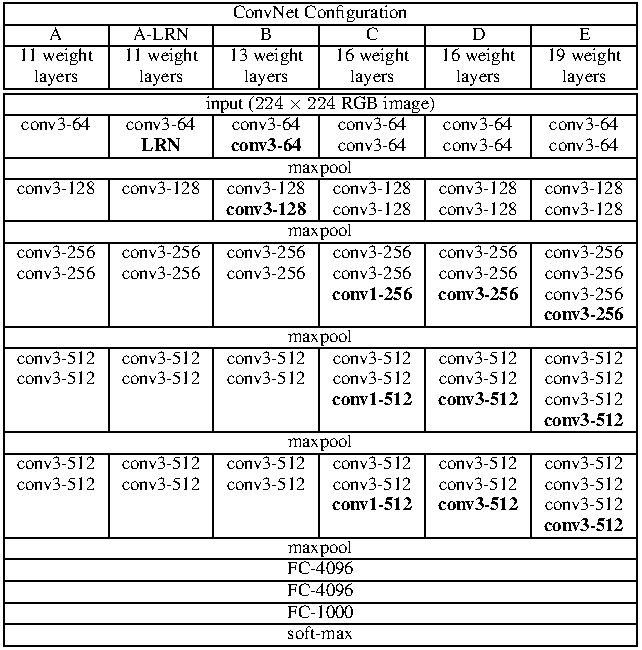
\includegraphics[width=0.8\textwidth]{Bilder/vgg16-architecture.pdf} 
	\caption{Die ursprünglichen VGG-Architekturen. Spalte D zeigt VGG16 wie in \autoref{sec:pretrained-backbones:vgg16} beschrieben. Abb. aus \cite{Simonyan.04092014}.}
	\label{fig:vgg16-architecture}
\end{figure} 

\begin{figure}
	\centering
	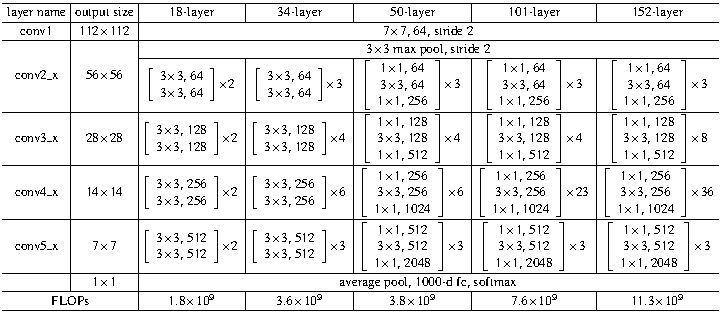
\includegraphics[width=0.8\textwidth]{Bilder/resnet34-architecture.pdf} 
	\caption{Die ursprünglichen ResNet-Architekturen. Zwischen jeweils zwei Convolutional-Layer befindet sich eine Skip-Connection \cite{He.10122015}.}
	\label{fig:resnet34-architecture}
\end{figure} 

\begin{figure}
	\centering
	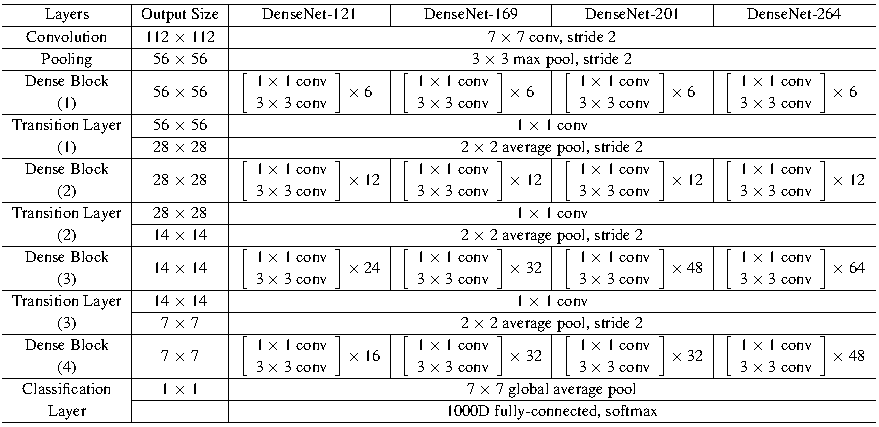
\includegraphics[width=0.8\textwidth]{Bilder/densenet121-architecture.pdf} 
	\caption{Die ursprünglichen DenseNet-Architekturen \cite{Huang.25082016}.}
	\label{fig:densenet121-architecture}
\end{figure} 

\begin{figure}
	\centering
	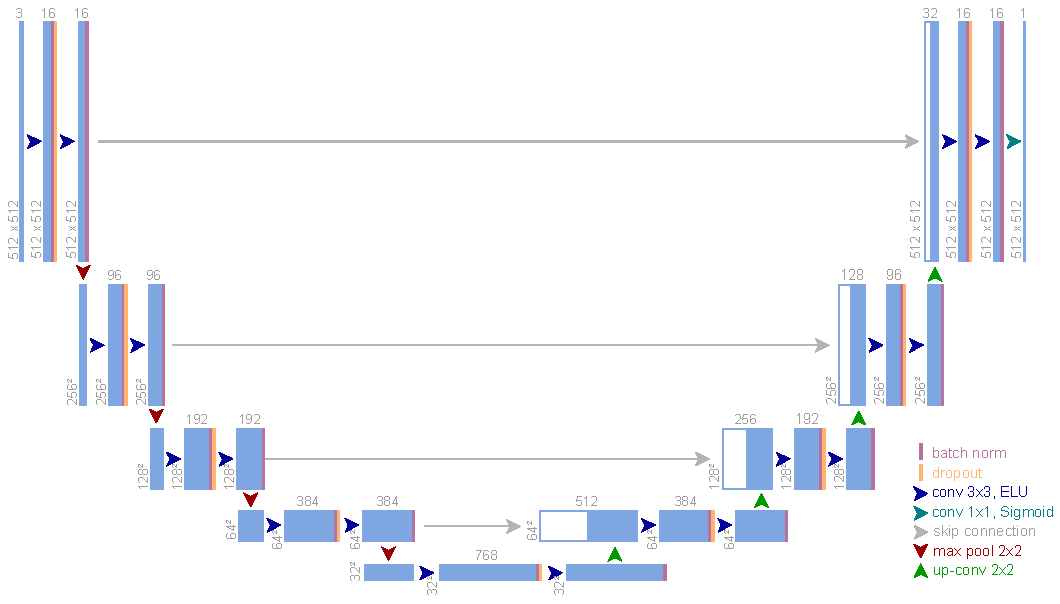
\includegraphics[width=1.\textwidth]{Bilder/own-unet-15mil.pdf} 
	\caption{Bike-U-Net-15 mit 15,165 Mio. Parametern.}
	\label{fig:bike-unet-15}
\end{figure} 

\pagebreak

\section{Quelltext-Implementation}

\lstinputlisting[
	label=code:quality,    % Label; genutzt für Referenzen auf dieses Code-Beispiel
	caption=Implementation des Quality-Maßes in Python zur Verwendung im Training und Testen von Keras-Modellen.,
	captionpos=b,               % Position, an der die Caption angezeigt wird t(op) oder b(ottom)
	style=EigenerPythonStyle,   % Eigener Style der vor dem Dokument festgelegt wurde
	firstline=1,                % Zeilennummer im Dokument welche als erste angezeigt wird
	lastline=50                 % Letzte Zeile welche ins LaTeX Dokument übernommen wird
]{Quellcode/quality.py}
%\clearpage
%\pagenumbering{Roman}  % römische Seitenzahlen für Anhang

\newpage
\end{document}
